\section{同调代数}

为了简化语言, 有时省略态射合成的 \(\circ\) 符号.

\subsection{Abel 范畴}

\subsubsection{加性范畴}

\begin{definition}[预加性范畴]
    一个预加性范畴是指 \(\mathbf{Ab}\) - 充实范畴,
    而加性函子是指 \(\mathbf{Ab}\) - 充实函子.
\end{definition}

\begin{definition}[加性范畴]
    一个加性范畴是一个预加性范畴, 若要求有零对象以及双积构造, 其自然构成一幺半范畴.
\end{definition}

\begin{remark}
    双积的定义如下, 对于两个对象 \(X_1,X_2\) 寻求一个对象 \(X_1 \oplus X_2 := Y\) 给出态射:

    \begin{center}
        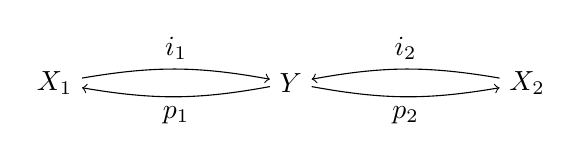
\begin{tikzpicture}
            \node (x1) at (-3,0) {\(X_1\)};
            \node (x2) at (3,0) {\(X_2\)};
            \node (y) at (0,0) {\(Y\)};

            \draw[->] (x1) to [bend left = 10] node[above] {\(i_1\)} (y);
            \draw[->] (x2) to [bend right = 10] node[above] {\(i_2\)} (y);
            \draw[->] (y) to [bend left = 10] node[below] {\(p_1\)} (x1);
            \draw[->] (y) to [bend right = 10] node[below] {\(p_2\)} (x2);
        \end{tikzpicture}
    \end{center}

    满足 \(p_1 \circ i_1 = \mathrm{id}_{X_1}, p_2 \circ i_2 = \mathrm{id}_{X_2}, i_1 \circ p_1 + i_2 \circ p_2 = \mathrm{id}_Y\).
\end{remark}

\begin{definition}[\(k\) 线性]
    一个 \(k\) - 线性范畴是指一个加性范畴 \(\mathcal{C}\), 其中的每个 \(\mathrm{hom}_{\mathcal{C}} (X,Y)\) 都是一个 \(k\) - 模,
    使得态射合成是 \(k\) - 线性的.

    亦定义 \(k\) - 线性函子.
\end{definition}

\begin{lemma}
    对于加性函子 \(F : \mathcal{C} \to \mathcal{D}\) 有同构 \(F(X) \oplus F(Y) \cong F(X \oplus Y)\).
\end{lemma}

\begin{lemma}
    \label {lemma:coproduct product biproduct are isomorphic}
    两个对象的双积, 积, 余积都是同构的.

    \begin{proof}
        给出双积 \(X_1 \oplus X_2\), 验证泛性质, 有双射 \((f_1,f_2) \mapsto i_1 \circ f_1 + i_2 \circ f_2 : \mathrm{hom}_{\mathcal{C}} (Y,X_1) \times \mathrm{hom}_{\mathcal{C}} (Y,X_2) \to \mathrm{hom}_{\mathcal{C}} (Y,X_1 \oplus X_2)\),
        \(f \mapsto (p_1 \circ f, p_2 \circ f) : \mathrm{hom}_{\mathcal{C}} (X_1 \oplus X_2,Y) \to \mathrm{hom}_{\mathcal{C}} (X_1,Y) \times \mathrm{hom}_{\mathcal{C}} (X_2,Y)\).

        亦有双射 \((f_1,f_2) \mapsto f_1 \circ p_1 + f_2 \circ p_2 : \mathrm{hom}_{\mathcal{C}} (X_1,Y) \times \mathrm{hom}_{\mathcal{C}} (X_2,Y) \to \mathrm{hom}_{\mathcal{C}} (X_1 \oplus X_2,Y)\),
        \(f \mapsto (f \circ i_1, f \circ i_2) : \mathrm{hom}_{\mathcal{C}} (Y,X_1 \oplus X_2) \to \mathrm{hom}_{\mathcal{C}} (Y,X_1) \times \mathrm{hom}_{\mathcal{C}} (Y,X_2)\).

        对称的, 如给出 \(X_1,X_2\) 的积 \(p_1,p_2 : X_1 \oplus X_2 \to X_1,X_2\),
        注意到 \(\mathrm{Hom}\) 总有 \(0\) 元, 考察 \(\mathrm{id}_{X_1},0 : X_1 \to X_1,X_2\),
        依泛性质给出 \(i_1 : X_1 \to X_1 \oplus X_2\), 亦有 \(i_2 : X_2 \to X_1 \oplus X_2\),
        验证知 \(i_1 \circ p_1 = \mathrm{id}_{X_1}, i_2 \circ p_2 = \mathrm{id}_{X_2}, p_1 \circ i_1 + p_2 \circ i_2 = \mathrm{id}_{X_1 \oplus X_2}\),

        给出 \(X_1,X_2\) 的余积 \(i_1,i_2 : X_1,X_2 \to X_1 \oplus X_2\), 亦可同理定义 \(p_1,p_2 : X_1 \oplus X_2 \to X_1,X_2\),
        验证知 \(i_1 \circ p_1 = \mathrm{id}_{X_1}, i_2 \circ p_2 = \mathrm{id}_{X_2}, p_1 \circ i_1 + p_2 \circ i_2 = \mathrm{id}_{X_1 \oplus X_2}\).
    \end{proof}
\end{lemma}

\begin{remark}
    循此思路, 有零对象的范畴 \(\mathcal{C}\) 给出嵌入 \(\coprod_{i \in I} X_i \to \prod_{i \in I} X_i\).
\end{remark}

\begin{lemma}
    一个预加性范畴的对象 \(X\) 是零对象当且仅当 \(X\) 是始对象或 \(X\) 是终对象或
    \(\mathrm{id}_X = 0\) 或 \(\mathrm{Hom} (X,X) = \{0\}\).
\end{lemma}

\subsubsection{子商像}

\begin{definition}
    范畴 \(\mathcal{C}\) 的一个对象 \(X\) 的子对象是指一个单态射 \(i : Y \to X\),
    定义商对象为一个满态射 \(p : X \to Z\), 全体子对象记作 \(\mathrm{Sub} (X)\), 全体商对象记作 \(\mathrm{Quot} (X)\).
\end{definition}

\begin{lemma}
    \label {lemma:injective combination is isomorphism}
    如果有单态射 \(a : X \to Y\), 若有 \(b : Y \to Z\) 使得 \(b \circ a\) 是同构, 则 \(a,b\) 是同构.

    \begin{proof}
        \(a \circ {(b \circ a)}^{-1} \circ b \circ a = a\) 故 \(a \circ {(b \circ a)}^{-1} \circ b = \mathrm{id}_Y\), \(b \circ a \circ {(b \circ a)}^{-1} = \mathrm{id}_X\),
        于是 \(a\) 亦是同构.
    \end{proof}
\end{lemma}

\begin{corollary}
    \label {corollary:surjective combination is isomorphism}
    如果有满态射 \(b : Y \to Z\) 使得 \(b \circ a\) 是同构, 则 \(a,b\) 是同构.
\end{corollary}

\begin{definition}
    \(\mathrm{Sub} (X)\) 与 \(\mathrm{Quot} (X)\) 上有自然的拟序关系, 定义子对象 \((Y_1,i_1) \leq (Y_2,i_2)\) 当且仅当存在态射 \(f : Y_1 \to Y_2\) 使得 \(i_2 \circ f = i_1\),
    定义商对象 \((Z_1,p_1) \leq (Z_2,p_2)\) 当且仅当存在态射 \(f : Z_1 \to Z_2\) 使得 \(p_2 = f \circ p_1\), 子对象 \((Y_1,i_1) \leq (Y_2,i_2) \leq (Y_1,i_1)\) 则 \((Y_1,i_1) \cong (Y_2,i_2)\),
    商对象 \((Z_1,p_1) \leq (Z_2,p_2) \leq (Z_1,p_1)\) 则 \((Z_1,p_1) \cong (Z_2,p_2)\).

    \begin{proof}
        \ref{lemma:injective combination is isomorphism} 与 \ref{corollary:surjective combination is isomorphism} 给出.
    \end{proof}
\end{definition}

\begin{lemma}
    有单态射 \(i : X \to Z\), 其关于 \(Y \to Z\) 拉回 \(i^\prime : X \times_Z Y \to Y\) 是单态射,
    对称的, 满态射推出亦满.

    \begin{proof}
        米田嵌入并且在 \(\mathbf{Set}\) 中验证即可.

        \begin{center}
            \begin{tikzpicture}
                \node (prod) at (-3,1) {\(\mathrm{Hom} (T,X \times_Z Y)\)};
                \node (X) at (3,1) {\(\mathrm{Hom} (T,X)\)};
                \node (Y) at (-3,-1) {\(\mathrm{Hom} (T,Y)\)};
                \node (Z) at (3,-1) {\(\mathrm{Hom} (T,Z)\)};
                \draw[->] (X) to (Z);
                \draw[->] (Y) to (Z);
                \draw[->] (prod) to (X);
                \draw[->] (prod) to (Y);
                \node at (0,0) {\(\Box\)};
            \end{tikzpicture}
        \end{center}
    \end{proof}
\end{lemma}

\begin{lemma}
    一族单态射 \(f_i : X_i \to Z\) 的直积 \(\prod_{i \in I} X_i \to Z\) 亦单, 对称的, 满态射余积 \(Z \to \coprod_{i \in I} X_i\) 亦满.

    \begin{proof}
        依旧米田嵌入并且在 \(\mathbf{Set}\) 中验证.
    \end{proof}
\end{lemma}

\begin{definition}
    子对象的商对象称为子商, 商对象的子对象称为商子.
\end{definition}

\begin{lemma}
    \(\mathcal{C}\) 有纤维积, 纤维余积, 单态射推出单, 满态射拉回满, 则子商与商子等价.

    \begin{proof}
        仅证明子商诱导出商子, 商子诱导出子商是对称的, 给出满射 \(p : Y \to X\), 单射 \(i : Y \to Z\),
        则有单射 \(X \to X \sqcup_Y Z\), 满射 \(Z \to X \sqcup_Y Z\).
    \end{proof}
\end{lemma}

\begin{definition}
    假定对于 \(f : X \to Y\) 存在 \(Y \sqcup_X Y\), 且两个 \(Y \to Y \sqcup_X Y\) 的等化子存在, 则称此等化子为 \(f\) 的像 \(\mathrm{im} f\).

    对称的余等化子 \(X \times_Y X \to X\) 称为 \(f\) 的余像 \(\mathrm{coim} f\).

    像带有典范单态射 \(\mathrm{im} f \to Y\), 余像带有典范满态射 \(X \to \mathrm{coim} f\).
\end{definition}

\begin{definition}
    可以典范的诱导出态射 \(\mathrm{coim} f \to \mathrm{im} f\), 若对于每个态射, 对应的像与余像均存在且总是同构, 则称其为严格范畴.
\end{definition}

\begin{lemma}
    \(f\) 的像和余像有如下的泛性质, 对于任意单态射 \(j : Y^\prime \to Y\) 且 \(f = j \circ g\), 则有唯一 \(\overline{g}\) 使得下图交换,
    对称的, 对于任意满态射 \(p : X \to X^\prime\) 且 \(f = g \circ p\), 则有唯一 \(\overline{g}\) 使得下图交换:

    \begin{center}
        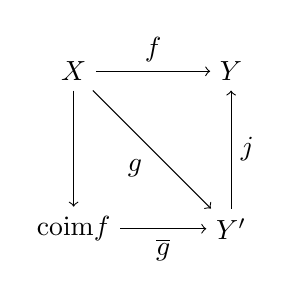
\begin{tikzpicture}
            \node (X) at (-1,1) {\(X\)};
            \node (Y) at (1,1) {\(Y\)};
            \node (Yp) at (1,-1) {\(Y^\prime\)};
            \node (coim) at (-1,-1) {\(\mathrm{coim} f\)};

            \draw[->] (X) to node[above] {\(f\)} (Y);
            \draw[->] (X) to node[below left] {\(g\)} (Yp);
            \draw[->] (Yp) to node[right] {\(j\)} (Y);
            \draw[->] (X) to (coim);
            \draw[->] (coim) to node[below] {\(\overline{g}\)} (Yp);
        \end{tikzpicture} 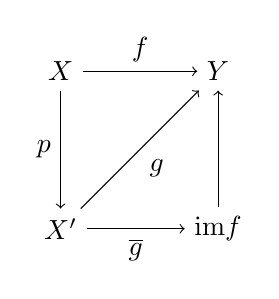
\begin{tikzpicture}
            \node (X) at (-1,1) {\(X\)};
            \node (Y) at (1,1) {\(Y\)};
            \node (Xp) at (-1,-1) {\(X^\prime\)};
            \node (im) at (1,-1) {\(\mathrm{im} f\)};

            \draw[->] (X) to node[above] {\(f\)} (Y);
            \draw[->] (X) to node[left] {\(p\)} (Xp);
            \draw[->] (Xp) to node[below right] {\(g\)} (Y);
            \draw[->] (Xp) to node[below] {\(\overline{g}\)} (im);
            \draw[->] (im) to (Y);
        \end{tikzpicture}
    \end{center}

    \begin{proof}
        \(j\) 单则两个 \(X \times_Y X \to X \to Y^\prime\) 的态射相等, 依余等化子的泛性质有 \(\overline{g}\), 对称亦然.
    \end{proof}
\end{lemma}

\begin{lemma}
    \label {lemma:mono iff coim is isomorphic to X}
    若存在所论的像和余像, \(f : X \to Y\) 是单态射当且仅当 \(\mathrm{coim} f \cong X\), 是满态射当且仅当 \(\mathrm{im} f \cong Y\).

    \begin{proof}
        在定义中依 \(f\) 单性可将其约去, 同一个态射的余等化子就是其像 \(X\), 若 \(\mathrm{coim} (f) \cong X\), 则任意 \(f_1,f_2 : L \to X\) 均可延伸至 \(L \to X \times_Y X \to X\) 的合成,
        对称亦然.
    \end{proof}
\end{lemma}

\begin{lemma}
    对于严格范畴中同构 \(f\), \(f\) 是同构当且仅当 \(f\) 既单又满.

    \begin{proof}
        在泛性质中取 \(Y^\prime = X\), \(X^\prime = Y\), 得到同构 \(X \cong \mathrm{coim} f \cong \mathrm{im} f \cong Y\).
    \end{proof}
\end{lemma}

\begin{remark}
    上述证明中蕴涵了下述结论:

    当态射典范选取时, \(f\) 满当且仅当 \(\mathrm{im} f \cong Y\), \(f\) 单当且仅当 \(\mathrm{coim} f \cong X\).
\end{remark}

\begin{lemma}
    严格范畴 \(f : X \to Y\) 的满单分解 \(X \twoheadrightarrow C \hookrightarrow Y\) 均同构.

    \begin{proof}
        有交换图表如下, 取态射 \(X \to C \to Y = X \to C \to \mathrm{im} f \to \mathrm{coim} f \to C \to Y\), 用单满性消去知 \(C \cong \mathrm{im} f \cong \mathrm{coim} f\).
        \begin{center}
            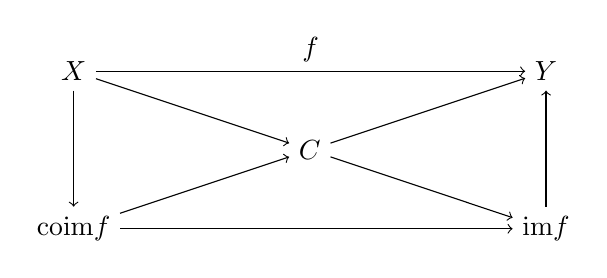
\begin{tikzpicture}
                \node (X) at (-3,1) {\(X\)};
                \node (Y) at (3,1) {\(Y\)};
                \node (C) at (0,0) {\(C\)};
                \node (coim) at (-3,-1) {\(\mathrm{coim} f\)};
                \node (im) at (3,-1) {\(\mathrm{im} f\)};

                \draw[->] (X) to node[above] {\(f\)} (Y);
                \draw[->] (X) to (coim); \draw[->] (im) to (Y); \draw[->] (coim) to (im);
                \draw[->] (X) to (C); \draw[->] (C) to (Y); \draw[->] (coim) to (C); \draw[->] (C) to (im);
            \end{tikzpicture}
        \end{center}
    \end{proof}
\end{lemma}

\subsubsection{Abel 范畴}

\begin{lemma}
    在加性范畴中, \(f + g : X \to Y\) 可以解释为下图的合成:

    \begin{center}
        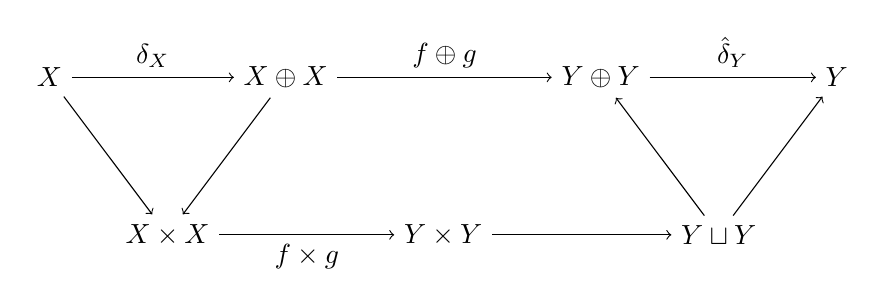
\begin{tikzpicture}
            \node (X) at (-5,1) {\(X\)};
            \node (X2) at (-2,1) {\(X \oplus X\)};
            \node (Y2) at (2,1) {\(Y \oplus Y\)};
            \node (Y) at (5,1) {\(Y\)};
            \node (xtx) at (-3.5,-1) {\(X \times X\)};
            \node (yty) at (0,-1) {\(Y \times Y\)};
            \node (ycy) at (3.5,-1) {\(Y \sqcup Y\)};

            \draw[->] (X) to node[above] {\(\delta_X\)} (X2);
            \draw[->] (X2) to node[above] {\(f \oplus g\)} (Y2);
            \draw[->] (Y2) to node[above] {\(\hat{\delta}_Y\)} (Y);
            \draw[->] (X) to (xtx); \draw[->] (yty) to (ycy); \draw[->] (ycy) to (Y);
            \draw[->] (xtx) to node[below] {\(f \times g\)} (yty);
            \draw[->] (X2) to (xtx); \draw[->] (ycy) to (Y2);
        \end{tikzpicture}
    \end{center}

    \begin{proof}
        图表的交换性给出 \(\delta_X, \hat{\delta}_Y\), \(f \oplus g := i_1^Y f p_1^X + i_2^Y g p_2^X\),
        依赖于 \(X \oplus Y\) 和 \(X \times X\) 间同构的给出给出了梯形的交换, 计算有 \((p_1^Y + p_2^Y) \circ (f \oplus g) \circ \delta_X = f + g\).
    \end{proof}
\end{lemma}

\begin{corollary}
    若一个加性范畴间的函子 \(F\) 保零对象和双积, 则其加性, 同理, 范畴等价, 伴随对总是给出加性函子.
\end{corollary}

\begin{definition}
    定义一个态射的核为其与 \(0\) 的等化子, 定义一个态射的余核为其与 \(0\) 的余等化子.
\end{definition}

\begin{definition}[Abel 范畴]
    一个 Abel 范畴是所有态射皆严格的加性范畴.
\end{definition}

\begin{lemma}
    对于任意范畴 \(I\), Abel 范畴 \(\mathcal{A}\) 的函子范畴 \(\mathcal{A}^I\) 亦为 Abel 范畴.

    \begin{proof}
        只需逐点给出 \(\mathrm{ker}, \mathrm{coker}\), 以及 \(\mathrm{im}, \mathrm{coim}\) 即可.
    \end{proof}
\end{lemma}

\subsection{若干图表引理}

本节用 \(=\) 表示同构, 均在 Abel 范畴中讨论, 常略去 \(\mathrm{im},\mathrm{coim}\) 的差别.

\subsubsection{基础引理}

\begin{lemma}
    \label {lemma:composition of kernels,cokernels and images,coimages}
    给出 \(f : X \to Y\), 则存在满足以下条件的图表:

    \begin{center}
        \begin{tikzpicture}
            \node (K) at (-4,0) {\(K\)};
            \node (X) at (-2,0) {\(X\)};
            \node (I) at (0,0) {\(I\)};
            \node (Y) at (2,0) {\(Y\)};
            \node (C) at (4,0) {\(C\)};

            \draw[->] (K) to node[above] {\(k\)} (X); \draw[->] (X) to node[above] {\(i\)} (I);
            \draw[->] (I) to node[above] {\(j\)} (Y); \draw[->] (Y) to node[above] {\(c\)} (C);
        \end{tikzpicture}
    \end{center}

    \begin{enumerate}
        \item \(j i = f\)
        \item \((K,k) = \mathrm{ker} (f)\), \((C,c) = \mathrm{coker} (f)\)
        \item \((I,i) = \mathrm{coker} (k)\), \((I,j) = \mathrm{ker} (c)\)
    \end{enumerate}

    \begin{proof}
        依 Abel 范畴的要求, 令 \(I = \mathrm{im} (f) = \mathrm{coim} (f), K = \mathrm{ker} (i),C = \mathrm{coker} (j)\),
        则 \(j i = f, (K,k) = \mathrm{ker} (f), (C,c) = \mathrm{coker} (f)\) 显然, 只需证明 \((I,i) = \mathrm{coker} (k), (I,j) = \mathrm{ker} (c)\),
        为此注意到 \(K \to X \times_Y X\) 单, 故 \(X \times_Y X \to X,K \to X\) 给出同样的余核, \((I,j)\) 侧亦然.
    \end{proof}
\end{lemma}

\begin{lemma}
    一个态射 \(f:X \to Y\) 单当且仅当 \(\mathrm{ker} (f) = 0,\mathrm{im} (f) = \mathrm{coim} (f) = X\), 满当且仅当 \(\mathrm{coker} (f) = 0,\mathrm{im} (f) = \mathrm{coim} (f) = Y\).

    \begin{proof}
        有关 \(\mathrm{im},\mathrm{coim}\) 的论断见 \ref{lemma:mono iff coim is isomorphic to X} 即可, 
        而注意到 \(f = g \iff f - g = 0\) 即证明了 \(\mathrm{ker} (f) = 0 \iff f\) 单, \(\mathrm{coker} (f) = 0 \iff f\) 满的论断.
    \end{proof}
\end{lemma}

\begin{definition}[复形]
    给出图表 \(X_\bullet\) 如下, 其称作复形 (complex) 若 \(d_{n+1} d_n = 0\).

    \begin{center}
        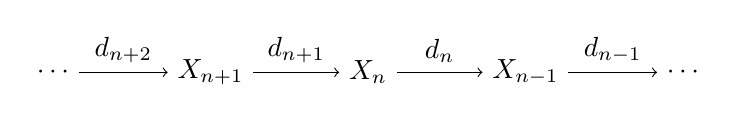
\begin{tikzpicture}
            \node (n+2) at (-4,0) {\(\cdots\)};
            \node (n+1) at (-2,0) {\(X_{n+1}\)};
            \node (n) at (0,0) {\(X_n\)};
            \node (n-1) at (2,0) {\(X_{n-1}\)};
            \node (n-2) at (4,0) {\(\cdots\)};

            \draw[->] (n+2) to node[above] {\(d_{n+2}\)} (n+1);
            \draw[->] (n+1) to node[above] {\(d_{n+1}\)} (n);
            \draw[->] (n) to node[above] {\(d_n\)} (n-1);
            \draw[->] (n-1) to node[above] {\(d_{n-1}\)} (n-2);
        \end{tikzpicture}
    \end{center}
\end{definition}

\begin{definition}[正合]
    一个复形 \(X_\bullet\) 称在 \(X_n\) 处正合 (exact) 当且仅当 \(\mathrm{im} (d_{n+1}) = \mathrm{ker} (d_n)\),
    若一个复形在每个 \(n\) 处都正合, 则称其为正合列.
\end{definition}

\begin{definition}[短正合列]
    考察如下复形, 若其正合, 则称其为短正合列 (short exact sequence):

    \begin{center}
        \begin{tikzpicture}
            \node (01) at (-4,0) {\(0\)};
            \node (X) at (-2,0) {\(X\)};
            \node (Y) at (0,0) {\(Y\)};
            \node (Z) at (2,0) {\(Z\)};
            \node (02) at (4,0) {\(0\)};

            \draw[->] (01) to (X); \draw[->] (X) to (Y); \draw[->] (Y) to (Z); \draw[->] (Z) to (02);
        \end{tikzpicture}
    \end{center}
\end{definition}

\begin{lemma}
    \label {lemma:coker of combination is a pushout}
    给出以下图表, 则右侧四边形为推出图表:

    \begin{center}
        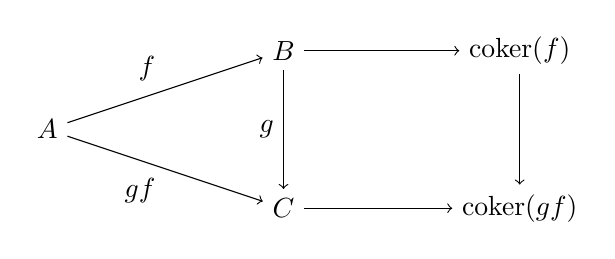
\begin{tikzpicture}
            \node (A) at (-3,0) {\(A\)};
            \node (B) at (0,1) {\(B\)};
            \node (C) at (0,-1) {\(C\)};
            \node (cokerf) at (3,1) {\(\mathrm{coker} (f)\)};
            \node (cokergf) at (3,-1) {\(\mathrm{coker} (gf)\)};

            \draw[->] (A) to node[above left] {\(f\)} (B); \draw[->] (A) to node[below left] {\(gf\)} (C); \draw[->] (B) to node[left] {\(g\)} (C);
            \draw[->] (B) to (cokerf); \draw[->] (cokerf) to (cokergf); \draw[->] (C) to (cokergf);
        \end{tikzpicture}
    \end{center}

    \begin{proof}
        验证 \(\mathrm{coker} (f) \sqcup_B C\) 满足 \(\mathrm{coker} (gf)\) 的泛性质即可.
    \end{proof}
\end{lemma}

\begin{lemma}
    \label {lemma:ker of combination is a pullback}
    对称的, \(\mathrm{ker} (g) \times_B A = \mathrm{ker} (gf)\).

    \begin{center}
        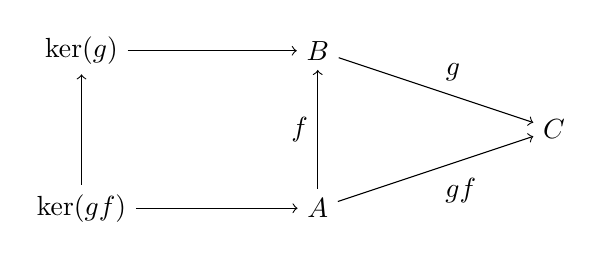
\begin{tikzpicture}
            \node (kerg) at (-3,1) {\(\mathrm{ker} (g)\)};
            \node (kergf) at (-3,-1) {\(\mathrm{ker} (gf)\)};
            \node (A) at (0,-1) {\(A\)};
            \node (B) at (0,1) {\(B\)};
            \node (C) at (3,0) {\(C\)};

            \draw[->] (kerg) to (B); \draw[->] (kergf) to (A); \draw[->] (kergf) to (kerg);
            \draw[->] (A) to node[left] {\(f\)} (B); \draw[->] (B) to node[above right] {\(g\)} (C); \draw[->] (A) to node[below right] {\(gf\)} (C);
        \end{tikzpicture}
    \end{center}
\end{lemma}

\begin{lemma}
    给出 Abel 范畴中的拉回图表 \(X = X^\prime \times_{Y^\prime} Y\), 则 \(\mathrm{ker} (f) \to \mathrm{ker} (f^\prime)\) 是同构.

    \begin{center}
        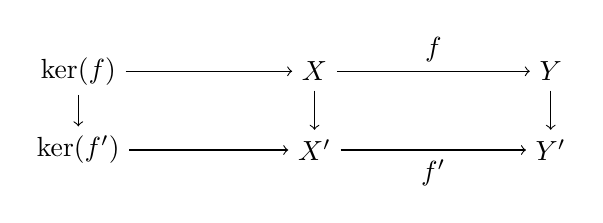
\begin{tikzpicture}
            \node (X) at (0,.5) {\(X\)};
            \node (Y) at (3,.5) {\(Y\)};
            \node (Xp) at (0,-.5) {\(X^\prime\)};
            \node (Yp) at (3,-.5) {\(Y^\prime\)};
            \node (kerf) at (-3,.5) {\(\mathrm{ker} (f)\)};
            \node (kerfp) at (-3,-.5) {\(\mathrm{ker} (f^\prime)\)};

            \draw[->] (X) to node[above] {\(f\)} (Y); \draw[->] (Xp) to node[below] {\(f^\prime\)} (Yp);
            \draw[->] (X) to (Xp); \draw[->] (Y) to (Yp); \draw[->] (kerf) to (X); \draw[->] (kerfp) to (Xp); \draw[->] (kerf) to (kerfp);
        \end{tikzpicture}
    \end{center}

    \begin{proof}
        依赖拉回给出 \(\mathrm{ker} (f^\prime) \to X\), 验证 \(\mathrm{ker} (f^\prime)\) 作为 \(\mathrm{ker} (f)\) 的泛性质.
    \end{proof}
\end{lemma}

\begin{remark}
    推出图表给出 \(\mathrm{coker}\) 的同构.
\end{remark}

\begin{lemma}
    给出 Abel 范畴中的拉回图表, 且 \(f^\prime\) 满, 则亦为推出图表, 且 \(f\) 满.

    \begin{center}
        \begin{tikzpicture}
            \node (X) at (-2,.5) {\(X\)};
            \node (Y) at (2,.5) {\(Y\)};
            \node (Xp) at (-2,-.5) {\(X^\prime\)};
            \node (Yp) at (2,-.5) {\(Y^\prime\)};

            \draw[->] (X) to node[above] {\(f\)} (Y); \draw[->] (Xp) to node[below] {\(f^\prime\)} (Yp);
            \draw[->] (X) to (Xp); \draw[->] (Y) to (Yp);
        \end{tikzpicture}
    \end{center}

    \begin{proof}
        考察列 \(X \to Y \oplus X^\prime \to Y^\prime\), 由于 \(X^\prime \to Y \oplus X^\prime \to Y^\prime\) 满, 故 \(Y \oplus X^\prime \to Y^\prime\) 满,
        依赖拉回给出在 \(0 \to X \to Y \oplus X^\prime \to Y^\prime \to 0\) 且在 \(X,Y^\prime\) 处正合.

        再证明 \(f\) 满, 利用推出知 \(\mathrm{coker} (f) = \mathrm{coker} (f^\prime) = 0\).
    \end{proof}
\end{lemma}

\begin{remark}
    在 Abel 范畴中, 子商等于商子.
\end{remark}

\begin{lemma}
    \label {lemma:definition of homology in terms of cokernels and kernels}
    给出 \(f : A \to B,g : B \to C\), 若 \(g f = 0\), 考察对应图表:

    \begin{center}
        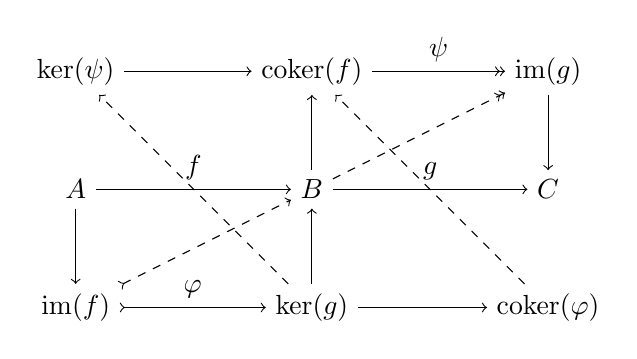
\begin{tikzpicture}
            \node (A) at (-3,0) {\(A\)};
            \node (B) at (0,0) {\(B\)};
            \node (C) at (3,0) {\(C\)};
            \node (imf) at (-3,-1.5) {\(\mathrm{im} (f)\)};
            \node (kerg) at (0,-1.5) {\(\mathrm{ker} (g)\)};
            \node (cokerf) at (0,1.5) {\(\mathrm{coker} (f)\)};
            \node (img) at (3,1.5) {\(\mathrm{im} (g)\)};
            \node (cokerphi) at (3,-1.5) {\(\mathrm{coker} (\varphi)\)};
            \node (kerpsi) at (-3,1.5) {\(\mathrm{ker} (\psi)\)};

            \draw[->] (A) to node[above] {\(f\)} (B); \draw[->] (B) to node[above] {\(g\)} (C);
            \draw[->] (A) to (imf); \draw[->] (kerg) to (B); \draw[->] (B) to (cokerf); \draw[->] (img) to (C);
            \draw[>->] (imf) to node[above] {\(\varphi\)} (kerg); \draw[->>] (cokerf) to node[above] {\(\psi\)} (img);
            \draw[->] (kerg) to (cokerphi); \draw[->] (kerpsi) to (cokerf);
            \draw[>->,dashed] (imf) to (B); \draw[->>,dashed] (B) to (img);
            \draw[->,dashed] (cokerphi) to (cokerf); \draw[->,dashed] (kerg) to (kerpsi);
        \end{tikzpicture}
    \end{center}

    则 \(\mathrm{ker} (g) \to \mathrm{coker} (f)\) 给出了两个满单分解, 分别透过 \(\mathrm{coker} (\varphi),\mathrm{ker} (\psi)\).

    \begin{proof}
        利用各处泛性质给出态射, 我们验证 \(\mathrm{coker} (\varphi) \to \mathrm{coker} (f)\) 单, 首先依赖 \(A \to \mathrm{im} (f)\) 满知 \(\mathrm{coker} (\varphi) = \mathrm{coker} (A \to \mathrm{ker} (g))\),
        利用 \ref{lemma:coker of combination is a pushout} 和上述引理即可知单性, 对称的, \(\mathrm{ker} (g) \to \mathrm{ker} (\psi)\) 满.
    \end{proof}
\end{lemma}

\begin{definition}[同调]
    给出 \(g f = 0\), 则定义 \(H [A \to B \to C] = \mathrm{coker} (\varphi) = \mathrm{ker} (\psi)\) 称同调 (homology).
\end{definition}

\begin{definition}
    对于复形 \(X_\bullet\), 定义其 \(n\) 阶同调 \(H_n (X_\bullet) = H[X_{n+1} \xrightarrow{d_{n+1}} X_n \xrightarrow{d_{n}} X_{n-1}]\).
\end{definition}

\begin{definition}
    对称定义上链复形 \(X^\bullet\) 如下:

    \begin{center}
        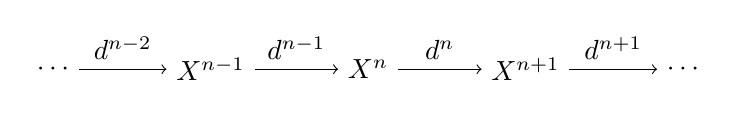
\begin{tikzpicture}
            \node (n-2) at (-4,0) {\(\cdots\)};
            \node (n-1) at (-2,0) {\(X^{n-1}\)};
            \node (n) at (0,0) {\(X^n\)};
            \node (n+1) at (2,0) {\(X^{n+1}\)};
            \node (n+2) at (4,0) {\(\cdots\)};

            \draw[->] (n-2) to node[above] {\(d^{n-2}\)} (n-1);
            \draw[->] (n-1) to node[above] {\(d^{n-1}\)} (n);
            \draw[->] (n) to node[above] {\(d^n\)} (n+1);
            \draw[->] (n+1) to node[above] {\(d^{n+1}\)} (n+2);
        \end{tikzpicture}
    \end{center}

    定义上同调 (cohomology) \(H^n (X^\bullet) = H[X^{n+1} \xrightarrow{d^{n+1}} X^n \xrightarrow{d^{n}} X^{n-1}]\).
\end{definition}

\begin{corollary}
    \(A \to B \to C\) 在 \(B\) 处正合当且仅当 \(H [A \to B \to C] = 0\), 故正合亦称为零调.

    \begin{proof}
        \(\varphi\) 单来自 \(\mathrm{im} (f) \to B\) 单, 满来自 \(\mathrm{coker} (\varphi) = 0\).
    \end{proof}
\end{corollary}

\begin{corollary}
    \(A \to B \to C\) 正合当且仅当 \(\mathrm{coker} (f) = \mathrm{im} (g)\).

    \begin{proof}
        \(\psi\) 单来自 \(\mathrm{ker} (\psi) = 0\), 满来自 \(B \to \mathrm{im} (g)\) 满.
    \end{proof}
\end{corollary}

\begin{definition}
    对复形 \(X^\bullet, Y^\bullet\), 可以定义 \(X^\bullet \to Y^\bullet\) 为形如 \(f^n : X^n \to Y^n\) 的态射, 使得 \(f^{n+1} d^n = d^n f^n\),
    其上有自然的加性结构 \({(f + g)}^n = f^n + g^n\), 以及复合结构 \({(g f)}^n = g^n f^n\).
\end{definition}

\begin{remark}
    记 \(\mathcal{A}\) 上全体复形及态射构成的范畴为 \(\mathbf{C} (\mathcal{A})\), 可被视作 \(\mathcal{A}^{\mathbb{Z}}\) 的子范畴,
    忘却函子记作 \(U : \mathbf{C} (\mathcal{A}) \to \mathcal{A}^{\mathbb{Z}}\).
\end{remark}

\begin{definition}[分次对象]
    \setlabel {分次对象}
    \label {definition:graded object}
    定义 \(\mathbb{Z}\) - 分次对象 (graded object) 为 \(\mathcal{A}^\mathbb{Z}\), 其带有自然的平移函子 \(T : \mathcal{A}^\mathbb{Z} \to \mathcal{A}^\mathbb{Z}\), 使得 \(T^n X = X^{n+1}\),
    同理可定义 \(\mathbb{Z}^m\) - 分次对象, 与自然的平移函子 \(T_1, T_2, \cdots, T_m\).
\end{definition}

\begin{remark}
    上链复形即为 \(\mathbb{Z}\) - 分次对象且给出了 \(d : X \to TX\), 满足 \((Td) d = 0\),
    其间态射为 \(\mathcal{A}^\mathbb{Z}\) 的态射, 且与 \(d\) 交换 : \((Tf) d = d f\).
\end{remark}

\begin{lemma}
    假使给出交换图表如下, 且 \(gf = 0,g^\prime f^\prime = 0\),

    \begin{center}
        \begin{tikzpicture}
            \node (A) at (-3,1) {\(A\)};
            \node (B) at (0,1) {\(B\)};
            \node (C) at (3,1) {\(C\)};
            \node (Ap) at (-3,-1) {\(A^\prime\)};
            \node (Bp) at (0,-1) {\(B^\prime\)};
            \node (Cp) at (3,-1) {\(C^\prime\)};

            \draw[->] (A) to node[above] {\(f\)} (B); \draw[->] (B) to node[above] {\(g\)} (C);
            \draw[->] (Ap) to node[below] {\(f^\prime\)} (Bp); \draw[->] (Bp) to node[below] {\(g^\prime\)} (Cp);
            \draw[->] (A) to (Ap); \draw[->] (B) to (Bp); \draw[->] (C) to (Cp);
        \end{tikzpicture}
    \end{center}

    则给出了唯一的 \(H [A \to B \to C] \to H [A^\prime \to B^\prime \to C^\prime]\), 使得有如下交换图表:
    
    \begin{center}
        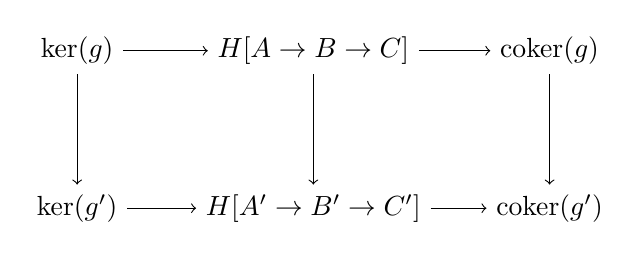
\begin{tikzpicture}
            \node (kerg) at (-3,1) {\(\mathrm{ker} (g)\)};
            \node (h) at (0,1) {\(H [A \to B \to C]\)};
            \node (cokerf) at (3,1) {\(\mathrm{coker} (g)\)};
            \node (kergp) at (-3,-1) {\(\mathrm{ker} (g^\prime)\)};
            \node (hp) at (0,-1) {\(H [A^\prime \to B^\prime \to C^\prime]\)};
            \node (cokerfp) at (3,-1) {\(\mathrm{coker} (g^\prime)\)};

            \draw[->] (kerg) to (h); \draw[->] (h) to (cokerf); \draw[->] (kergp) to (hp); \draw[->] (hp) to (cokerfp);
            \draw[->] (kerg) to (kergp); \draw[->] (h) to (hp); \draw[->] (cokerf) to (cokerfp);
        \end{tikzpicture}
    \end{center}

    \begin{proof}
        依赖 \(\varinjlim,\varprojlim,\oplus\) 的函子性, 唯一性约化到泛性质给出的左右两侧态射的唯一性与左侧水平态射的满性,
        右侧水平态射的单性.
    \end{proof}
\end{lemma}

\begin{lemma}
    复形的极限可逐项构造, 任意给出 \(\alpha : I \to \mathbf{C}(\mathcal{A})\),
    若存在 \(\varinjlim U \alpha\), 则其唯一对应了 \(\varinjlim \alpha\), \(\varprojlim \alpha\) 亦然.

    \begin{proof}
        需在给出的 \(\varinjlim U \alpha\) 上给出对应的 \(d\), 注意到 \(d\) 给出了 \(\alpha \to T \alpha\) 的自然变换,
        而 \(\varinjlim T \alpha \cong T \varinjlim \alpha\), 依赖 \(\varinjlim\) 函子性给出了 \(\varinjlim \alpha \to \varinjlim T \alpha \cong T \varinjlim \alpha\).

        我们需验证上述构造在 \(\mathbf{C} (\mathcal{A})\) 上仍给出 \(\varinjlim\), 注意到泛性质给出 \(\mathcal{A}^\mathbb{Z}\) 中 \(\varinjlim \alpha \to T L\) 的唯一性.
    \end{proof}
\end{lemma}

\begin{corollary}
    若 \(\mathcal{A}\) 是 Abel 范畴, 则 \(\mathbf{C} (\mathcal{A})\) 亦是 Abel 范畴.
\end{corollary}

\begin{lemma}
    有恒等式 \(H [A \to B \to C] \oplus H [A^\prime \to B^\prime \to C^\prime] = H [A \oplus A^\prime \to B \oplus B^\prime \to C \oplus C^\prime]\).

    \begin{proof}
        利用 \(\oplus\) 函子性.
    \end{proof}
\end{lemma}

\begin{definition}[双复形]
    双复形代指 \(\mathcal{A}^{\mathbb{Z}^2}\) 上的对象, 其上有两个微分算子 \(d_1 : X \to T_1 X,d_2 : X \to T_2 X\), 满足方程

    \[
        \begin{aligned}
            (T_1 d_1) d_1 &= 0 \\
            (T_2 d_2) d_2 &= 0 \\
            (T_2 d_1) d_2 &= (T_1 d_2) d_1
        \end{aligned}
    \]

    可解作图表如下:

    \begin{center}
        \begin{tikzpicture}
            \node (pq+2) at (-1,3) {\(\vdots\)};
            \node (p+1q+2) at (1,3) {\(\vdots\)};
            \node (p-1q+1) at (-3,1) {\(\cdots\)};
            \node (pq+1) at (-1,1) {\(X^{p,q+1}\)};
            \node (p+1q+1) at (1,1) {\(X^{p+1,q+1}\)};
            \node (p+2q+1) at (3,1) {\(\cdots\)};
            \node (p-1q) at (-3,-1) {\(\cdots\)};
            \node (pq) at (-1,-1) {\(X^{p,q}\)};
            \node (p+1q) at (1,-1) {\(X^{p+1,q}\)};
            \node (p+2q) at (3,-1) {\(\cdots\)};
            \node (pq-1) at (-1,-3) {\(\vdots\)};
            \node (p+1q-1) at (1,-3) {\(\vdots\)};

            \draw[->] (p-1q+1) to (pq+1); \draw[->] (pq+1) to (p+1q+1); \draw[->] (p+1q+1) to (p+2q+1);
            \draw[->] (p-1q) to (pq); \draw[->] (pq) to (p+1q); \draw[->] (p+1q) to (p+2q);
            \draw[->] (pq-1) to (pq); \draw[->] (pq) to (pq+1); \draw[->] (pq+1) to (pq+2);
            \draw[->] (p+1q-1) to (p+1q); \draw[->] (p+1q) to (p+1q+1); \draw[->] (p+1q+1) to (p+1q+2);
        \end{tikzpicture}
    \end{center}
\end{definition}

\subsubsection{蝾螈引理}

\begin{lemma}
    \label {lemma:universal property of exactness}
    给出复形 \(X^\prime \xrightarrow{f} X \xrightarrow{g} X^{\prime\prime}\), 则其在 \(X\) 处正合当且仅当对于任何 \(g h = 0\) 的 \(h : S \to X\),
    存在 \(S^\prime \to S\) 满与 \(S^\prime \to X^\prime\) 下图交换:

    \begin{center}
        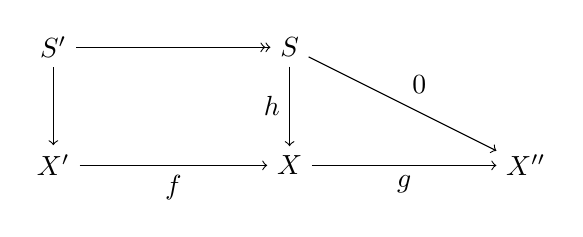
\begin{tikzpicture}
            \node (Sp) at (-3,.75) {\(S^\prime\)};
            \node (S) at (0,.75) {\(S\)};
            \node (Xp) at (-3,-.75) {\(X^\prime\)};
            \node (X) at (0,-.75) {\(X\)};
            \node (Xpp) at (3,-.75) {\(X^{\prime\prime}\)};

            \draw[->>] (Sp) to (S); \draw[->] (Xp) to node[below] {\(f\)} (X);
            \draw[->] (Sp) to (Xp); \draw[->] (S) to node[left] {\(h\)} (X);
            \draw[->] (X) to node[below] {\(g\)} (Xpp);
            \draw[->] (S) to node[above right] {\(0\)} (Xpp);
        \end{tikzpicture}
    \end{center}

    \begin{proof}
        \(\implies\) : 注意到 \(h,f\) 均可透过 \(\mathrm{ker} (g)\) 分解, 令 \(S^\prime = S \times_{\mathrm{ker}(g)} X^\prime\),
        注意到正合给出 \(X^\prime \to \mathrm{ker} (g) = \mathrm{im} (f)\) 满, 故 \(S^\prime \to S\) 满.

        \(\impliedby\) : 令 \(S = \mathrm{ker} (g)\), 则 \(S^\prime \to S\) 满意味着 \(X^\prime \to \mathrm{ker} (g)\) 满,
        这里 \(S^\prime \to X^\prime \to \mathrm{ker} (g) = S^\prime \to S\) 基于 \(\mathrm{ker} (g) \to X\) 单, 故 \(\mathrm{ker} (g)\) 给出满单分解, 同构于 \(\mathrm{im} (f)\) 即正合.
    \end{proof}
\end{lemma}

\begin{lemma}
    \label {lemma:universal property of exactness symmetric}
    对称的, 给出复形 \(X^\prime \xrightarrow{f} X \xrightarrow{g} X^{\prime\prime}\), 则其在 \(X\) 处正合当且仅当对于任何 \(h f = 0\) 的 \(h : X \to S\),
    存在 \(S \to S^\prime\) 单与 \(X^{\prime\prime} \to S^\prime\) 下图交换:

    \begin{center}
        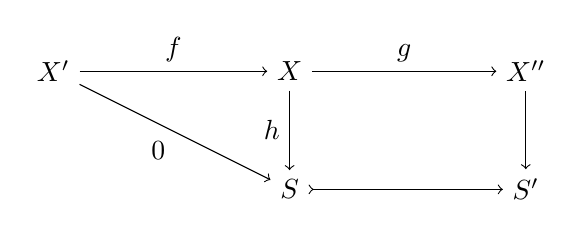
\begin{tikzpicture}
            \node (Xp) at (-3,.75) {\(X^\prime\)};
            \node (X) at (0,.75) {\(X\)};
            \node (Xpp) at (3,.75) {\(X^{\prime\prime}\)};
            \node (S) at (0,-.75) {\(S\)};
            \node (Sp) at (3,-.75) {\(S^\prime\)};

            \draw[->] (Xp) to node[above] {\(f\)} (X); \draw[->] (X) to node[above] {\(g\)} (Xpp);
            \draw[->] (X) to node[left] {\(h\)} (S); \draw[>->] (S) to (Sp);
            \draw[->] (Xpp) to (Sp);
            \draw[->] (Xp) to node[below left] {\(0\)} (S);
        \end{tikzpicture}
    \end{center}

    \begin{proof}
        \(\implies\) : 注意到 \(h,g\) 均可透过 \(\mathrm{coker} (f)\) 分解, 令 \(S^\prime = X^{\prime\prime} \times_{\mathrm{coker} (f)} S\),
        注意到正合给出 \(\mathrm{coker} (f) = \mathrm{im} (g) \to X^{\prime\prime}\) 单, 故 \(S^\prime \to X^{\prime\prime}\) 单.

        \(\impliedby\) : 令 \(S = \mathrm{coker} (f)\), 则 \(S \to S^\prime\) 单意味着 \(S \to X^{\prime\prime}\) 单, 这里 \(\mathrm{coker} (f) \to X^{\prime\prime} \to S^\prime = S \to S^\prime\) 基于 \(X \to \mathrm{coker} (f)\) 满, 故 \(\mathrm{coker} (f)\) 给出满单分解, 同构于 \(\mathrm{im} (g)\) 即正合.
    \end{proof}
\end{lemma}

\begin{definition}
    考察双复形中的子图如下:

    \begin{center}
        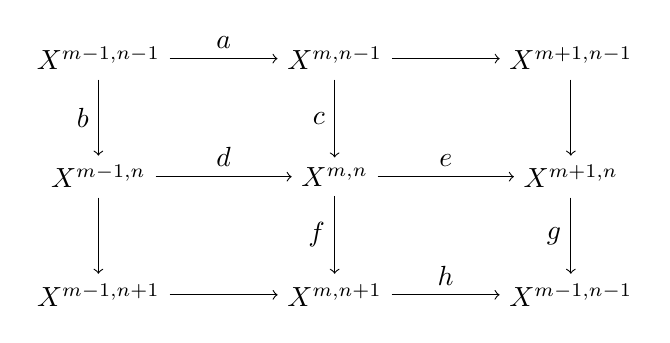
\begin{tikzpicture}
            \node (-1-1) at (-3,1.5) {\(X^{m-1,n-1}\)};
            \node (0-1) at (0,1.5) {\(X^{m,n-1}\)};
            \node (1-1) at (3,1.5) {\(X^{m+1,n-1}\)};
            \node (-10) at (-3,0) {\(X^{m-1,n}\)};
            \node (00) at (0,0) {\(X^{m,n}\)};
            \node (10) at (3,0) {\(X^{m+1,n}\)};
            \node (-11) at (-3,-1.5) {\(X^{m-1,n+1}\)};
            \node (01) at (0,-1.5) {\(X^{m,n+1}\)};
            \node (11) at (3,-1.5) {\(X^{m-1,n-1}\)};

            \draw[->] (-1-1) to node[above] {\(a\)} (0-1); \draw[->] (0-1) to (1-1);
            \draw[->] (-10) to node[above] {\(d\)} (00); \draw[->] (00) to node[above] {\(e\)} (10);
            \draw[->] (-11) to (01); \draw[->] (01) to node[above] {\(h\)} (11);
            \draw[->] (-1-1) to node[left] {\(b\)} (-10); \draw[->] (0-1) to node[left] {\(c\)} (00); \draw[->] (1-1) to (10);
            \draw[->] (-10) to (-11); \draw[->] (00) to node[left] {\(f\)} (01); \draw[->] (10) to node[left] {\(g\)} (11);
        \end{tikzpicture}
    \end{center}

    \begin{enumerate}
        \item 定义横向 (horizontal) 同调为 
            \[
                H^{m,n}_{h} (X) := H[X^{m-1,n} \xrightarrow{d} X^{m,n} \xrightarrow{e} X^{m+1,n}]
            \]
        \item 定义纵向 (vertical) 同调为
            \[
                H^{m,n}_{v} (X) := H[X^{m,n-1} \xrightarrow{c} X^{m,n} \xrightarrow{f} X^{m,n+1}]
            \]
        \item 定义受向 (receptor) 同调为
            \[
                H^{m,n}_{r} (X) := H[X^{m-1,n-1} \xrightarrow{ca = db} X^{m,n} \xrightarrow{(e,f)} X^{m+1,n} \times_{X^{m+1,n+1}} X^{m,n+1}]
            \]
        \item 定义施向 (donor) 同调为
            \[
                H^{m,n}_{d} (X) := H[X^{m-1,n} \sqcup_{X^{m-1,n-1}} X^{m,n-1} \xrightarrow{(d,c)} X^{m,n} \xrightarrow{ge = hf} X^{m+1,n+1}]
            \]
    \end{enumerate}
\end{definition}

\begin{lemma}
    有如下交换图表:

    \begin{center}
        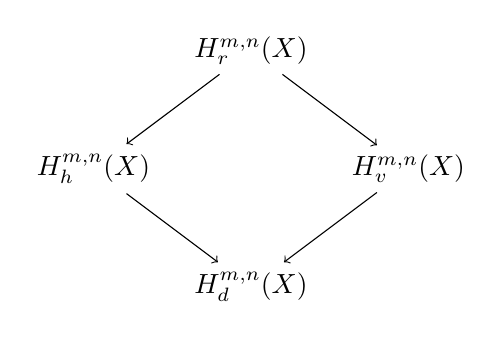
\begin{tikzpicture}
            \node (r) at (0,1.5) {\(H^{m,n}_{r} (X)\)};
            \node (h) at (-2,0) {\(H^{m,n}_{h} (X)\)};
            \node (v) at (2,0) {\(H^{m,n}_{v} (X)\)};
            \node (d) at (0,-1.5) {\(H^{m,n}_{d} (X)\)};

            \draw[->] (r) to (h); \draw[->] (r) to (v); \draw[->] (h) to (d); \draw[->] (v) to (d);
        \end{tikzpicture}
    \end{center}

    \begin{proof}
        给出复形的交换图表, 依赖其在同调上给出态射的唯一性即可.

        \begin{center}
            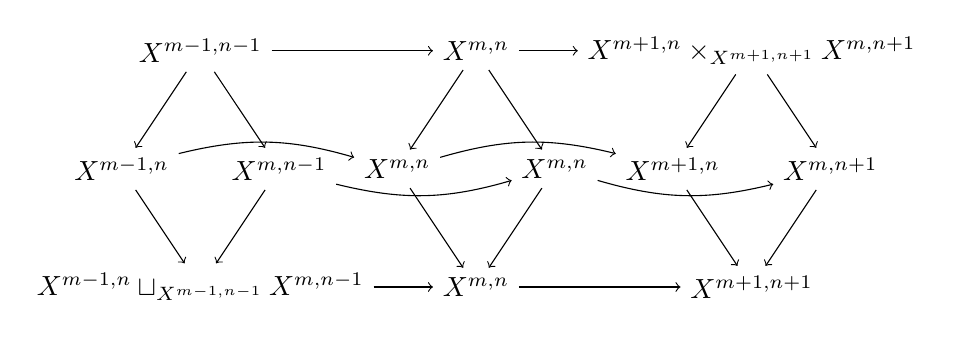
\begin{tikzpicture}
                \node (r1) at (-3.5,1.5) {\(X^{m-1,n-1}\)};
                \node (h1) at (-4.5,0) {\(X^{m-1,n}\)};
                \node (v1) at (-2.5,0) {\(X^{m,n-1}\)};
                \node (d1) at (-3.5,-1.5) {\(X^{m-1,n} \sqcup_{X^{m-1,n-1}} X^{m,n-1}\)};
                \node (r2) at (0,1.5) {\(X^{m,n}\)};
                \node (h2) at (-1,0) {\(X^{m,n}\)};
                \node (v2) at (1,0) {\(X^{m,n}\)};
                \node (d2) at (0,-1.5) {\(X^{m,n}\)};
                \node (r3) at (3.5,1.5) {\(X^{m+1,n} \times_{X^{m+1,n+1}} X^{m,n+1}\)};
                \node (h3) at (2.5,0) {\(X^{m+1,n}\)};
                \node (v3) at (4.5,0) {\(X^{m,n+1}\)};
                \node (d3) at (3.5,-1.5) {\(X^{m+1,n+1}\)};

                \draw[->] (r1) to (h1); \draw[->] (r1) to (v1); \draw[->] (h1) to (d1); \draw[->] (v1) to (d1);
                \draw[->] (r2) to (h2); \draw[->] (r2) to (v2); \draw[->] (h2) to (d2); \draw[->] (v2) to (d2);
                \draw[->] (r3) to (h3); \draw[->] (r3) to (v3); \draw[->] (h3) to (d3); \draw[->] (v3) to (d3);
                \draw[->] (r1) to (r2); \draw[->] (r2) to (r3);
                \draw[->,bend left = 15] (h1) to (h2); \draw[->,bend left = 15] (h2) to (h3);
                \draw[->,bend right = 15] (v1) to (v2); \draw[->,bend right = 15] (v2) to (v3);
                \draw[->] (d1) to (d2); \draw[->] (d2) to (d3);
            \end{tikzpicture}
        \end{center}
    \end{proof}
\end{lemma}

\begin{lemma}
    双复形中的一个态射 \(f = d^{m,n}_{\bullet} : X \to Y\) 给出了 \(H_{d} (X) \to H_{r} (Y)\).

    \begin{proof}
        仅以 \(X^{m,n} \to X^{m+1,n}\) 为例, 注意到 \(X^{m,n} \to X^{m+2,n} = 0,X^{m,n} \to X^{m+2,n+1} = 0\), 故有等式:
        
        \[
            \begin{aligned}
                \mathrm{ker} (X^{m,n} \to X^{m+1,n+1}) &= \mathrm{ker} (X^{m,n} \to X^{m+2,n} \times_{X^{m+2,n+1}} X^{m+1,n+1}) \\
                \mathrm{coker} (X^{m,n-1} \to X^{m+1,n}) &= \mathrm{coker} (X^{m-1,n} \sqcup_{X^{m-1,n-1}} X^{m,n-1} \to X^{m+1,n})
            \end{aligned}
        \]

        诱导出 \(\mathrm{ker},\mathrm{coker}\) 间的态射, 同调作为其满单分解, 自然也给出 \(H_{d}^{m,n} (X) \to H_{r}^{m+1,n} (Y)\).
    \end{proof}
\end{lemma}

\begin{lemma}
    \(H^{m,n}_{v} (X) \to H^{m+1,n}_{v} (X)\) 透过 \(H^{m,n}_{d} (X) \to H^{m+1,n}_{r} (X)\) 分解, 对称的 \(H^{m,n}_{h} (X) \to H^{m,n+1}_{h} (X)\) 透过 \(H^{m,n}_{r} (X) \to H^{m,n+1}_{d} (X)\) 分解.

    \begin{proof}
        以 \(H_v\) 为例, 将 \(\mathrm{ker},\mathrm{coker}\) 间的态射拉开, 得到以下交换图表:

        \begin{center}
            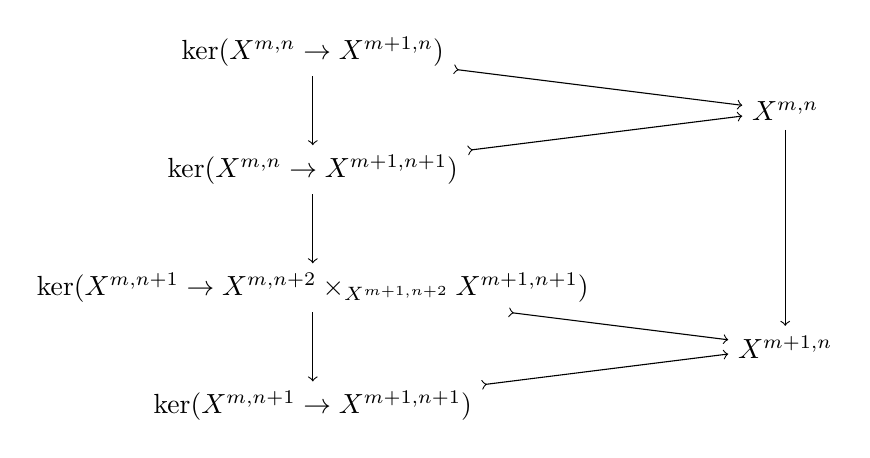
\begin{tikzpicture}
                \node (ker1) at (-3,2.25) {\(\mathrm{ker} (X^{m,n} \to X^{m+1,n})\)};
                \node (ker2) at (-3,0.75) {\(\mathrm{ker} (X^{m,n} \to X^{m+1,n+1})\)};
                \node (ker3) at (-3,-0.75) {\(\mathrm{ker} (X^{m,n+1} \to X^{m,n+2} \times_{X^{m+1,n+2}} X^{m+1,n+1})\)};
                \node (ker4) at (-3,-2.25) {\(\mathrm{ker} (X^{m,n+1} \to X^{m+1,n+1})\)};
                \node (X1) at (3,1.5) {\(X^{m,n}\)};
                \node (X2) at (3,-1.5) {\(X^{m+1,n}\)};

                \draw[>->] (ker1) to (X1); \draw[>->] (ker2) to (X1); \draw[>->] (ker3) to (X2); \draw[>->] (ker4) to (X2);
                \draw[->] (ker1) to (ker2); \draw[->] (ker2) to (ker3); \draw[->] (ker3) to (ker4);
                \draw[->] (X1) to (X2);
            \end{tikzpicture}

            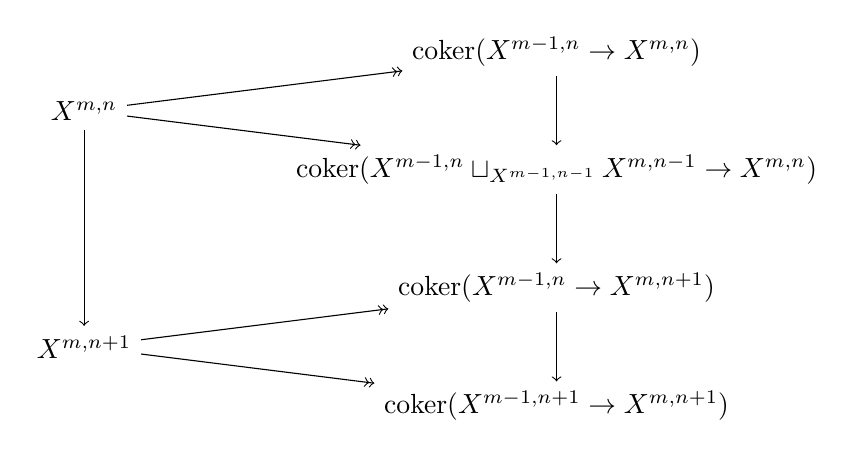
\begin{tikzpicture}
                \node (coker1) at (3,2.25) {\(\mathrm{coker} (X^{m-1,n} \to X^{m,n})\)};
                \node (coker2) at (3,0.75) {\(\mathrm{coker} (X^{m-1,n} \sqcup_{X^{m-1,n-1}} X^{m,n-1} \to X^{m,n})\)};
                \node (coker3) at (3,-0.75) {\(\mathrm{coker} (X^{m-1,n} \to X^{m,n+1})\)};
                \node (coker4) at (3,-2.25) {\(\mathrm{coker} (X^{m-1,n+1} \to X^{m,n+1})\)};
                \node (X1) at (-3,1.5) {\(X^{m,n}\)};
                \node (X2) at (-3,-1.5) {\(X^{m,n+1}\)};

                \draw[->>] (X1) to (coker1); \draw[->>] (X1) to (coker2); \draw[->>] (X2) to (coker3); \draw[->>] (X2) to (coker4);
                \draw[->] (coker1) to (coker2); \draw[->] (coker2) to (coker3); \draw[->] (coker3) to (coker4);
                \draw[->] (X1) to (X2);
            \end{tikzpicture}
        \end{center}

        注意到满足下图交换的虚线唯一, 对此满单分解也给出唯一的复合.

        \begin{center}
            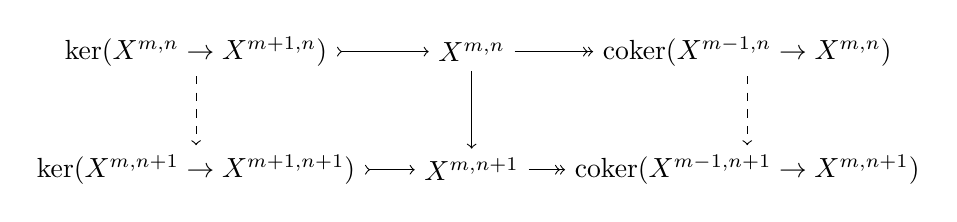
\begin{tikzpicture}
                \node (ker1) at (-3.5,.75) {\(\mathrm{ker} (X^{m,n} \to X^{m+1,n})\)};
                \node (ker2) at (-3.5,-.75) {\(\mathrm{ker} (X^{m,n+1} \to X^{m+1,n+1})\)};
                \node (X1) at (0,.75) {\(X^{m,n}\)};
                \node (X2) at (0,-.75) {\(X^{m,n+1}\)};
                \node (coker1) at (3.5,.75) {\(\mathrm{coker} (X^{m-1,n} \to X^{m,n})\)};
                \node (coker2) at (3.5,-.75) {\(\mathrm{coker} (X^{m-1,n+1} \to X^{m,n+1})\)};

                \draw[>->] (ker1) to (X1); \draw[>->] (ker2) to (X2); 
                \draw[->>] (X1) to (coker1); \draw[->>] (X2) to (coker2);
                \draw[->,dashed] (ker1) to (ker2); \draw[->,dashed] (coker1) to (coker2); \draw[->] (X1) to (X2);
            \end{tikzpicture}
        \end{center}
    \end{proof}
\end{lemma}

在引出蝾螈引理前, 我们先证明两个引理.

\begin{lemma}
    给出两个拉回图表并排放置, 则外框亦为拉回图表, 给出两个推出图表并排放置, 则外框亦为推出图表:

    \begin{center}
        \begin{tikzpicture}
            \node (A) at (-3,1.5) {\(A\)};
            \node (B) at (0,1.5) {\(B\)};
            \node (C) at (3,1.5) {\(C\)};
            \node (D) at (-3,0) {\(D\)};
            \node (E) at (0,0) {\(E\)};
            \node (F) at (3,0) {\(F\)};

            \draw[->] (A) to (B); \draw[->] (B) to (C);
            \draw[->] (D) to (E); \draw[->] (E) to (F);
            \draw[->] (D) to (A); \draw[->] (E) to (B); \draw[->] (F) to (C);
        \end{tikzpicture}
    \end{center}

    \begin{proof}
        验证泛性质即可.
    \end{proof}
\end{lemma}

\begin{lemma}
    \label {lemma:exact sequence's pullback and pushout}
    给出图表如下:

    \begin{center}
        \begin{tikzpicture}
            \node (H) at (0,2) {\(H\)};
            \node (P) at (-2,1) {\(P\)};
            \node (Q) at (2,1) {\(Q\)};
            \node (M) at (-4,0) {\(P \times_B A\)};
            \node (B) at (0,0) {\(B\)};
            \node (N) at (4,0) {\(Q \sqcup_B C\)};
            \node (A) at (-2,-1) {\(A\)};
            \node (C) at (2,-1) {\(C\)};

            \draw[->>] (P) to (H); \draw[>->] (H) to (Q);
            \draw[>->] (P) to (B); \draw[->>] (B) to (Q);
            \draw[->] (M) to (P); \draw[->] (Q) to (N);
            \draw[>->] (M) to (A); \draw[->>] (C) to (N);
            \draw[->] (A) to (B); \draw[->] (B) to (C);

            \node (pushout) at (2,0) {\(\boxplus\)};
            \node (pullback) at (-2,0) {\(\Box\)};
            \node (pp) at (0,1) {\(\boxplus (\iff \Box)\)};
        \end{tikzpicture}
    \end{center}

    若 \(A \to B \to C\) 正合, 则 \(P \times_B A \to S \to Q \sqcup_B C\) 亦正合.

    \begin{proof}
        任意给出 \(S \to H\), 注意到有 \((S \to Q,0) : S \to Q \oplus C\), 与正合列 \(B \to Q \oplus C \to Q \sqcup_B C\), 
        故存在 \(S^{\prime\prime} \to S\) 满与 \(S^{\prime\prime} \to B\), 其复合至 \(C\) 为透过 \(S\) 的 \(0\),
        故存在 \(S^\prime \to S^{\prime \prime}\) 满与 \(S^\prime \to A\), 其可透过 \(H \times_Q A = P \times_B A\) 分解.
    \end{proof}
\end{lemma}

\begin{lemma}[蝾螈引理]
    \setlabel {蝾螈引理}
    \label {lemma:salamander lemma}
    给出双复形中图表如下:

    \begin{center}
        \begin{tikzpicture}
            \node (C) at (-1.5,.75) {\(C\)};
            \node (A) at (0,.75) {\(A\)};
            \node (B) at (0,-.75) {\(B\)};
            \node (D) at (1.5,-.75) {\(D\)};
            \node (E) at (-3,2.25) {\(E\)};
            \node (F) at (-1.5,2.25) {\(F\)};
            \node (G) at (0,2.25) {\(G\)};
            \node (H) at (-3,.75) {\(H\)};
            \node (I) at (1.5,.75) {\(I\)};
            \node (J) at (-1.5,-.75) {\(J\)};
            \node (K) at (3,-.75) {\(K\)};
            \node (L) at (0,-2.25) {\(L\)};
            \node (M) at (1.5,-2.25) {\(M\)};
            \node (N) at (3,-2.25) {\(N\)};

            \draw[->] (E) to (F); \draw[->] (F) to (G); 
            \draw[->] (H) to (C); \draw[->] (C) to (A); \draw[->] (A) to (I);
            \draw[->] (J) to (B); \draw[->] (B) to (D); \draw[->] (D) to (K);
            \draw[->] (L) to (M); \draw[->] (M) to (N);
            \draw[->] (E) to (H); \draw[->] (F) to (C); \draw[->] (G) to (A);
            \draw[->] (C) to (J); \draw[->] (A) to (B); \draw[->] (I) to (D);
            \draw[->] (B) to (L); \draw[->] (D) to (M); \draw[->] (K) to (N);
        \end{tikzpicture}
    \end{center}

    则给出正合列如下, 其中态射皆为上述引理所诱导出的.

    \[
        H_d (C) \xrightarrow{H_r(A)} H_v (A) \to H_d(A) \to H_r(B) \to H_v (B) \xrightarrow{H_d (B)} H_r (D)
    \]

    \begin{proof}
        逐项施以验证, \(H_v (A)\) 处绘出图表如下:

        \begin{center}
            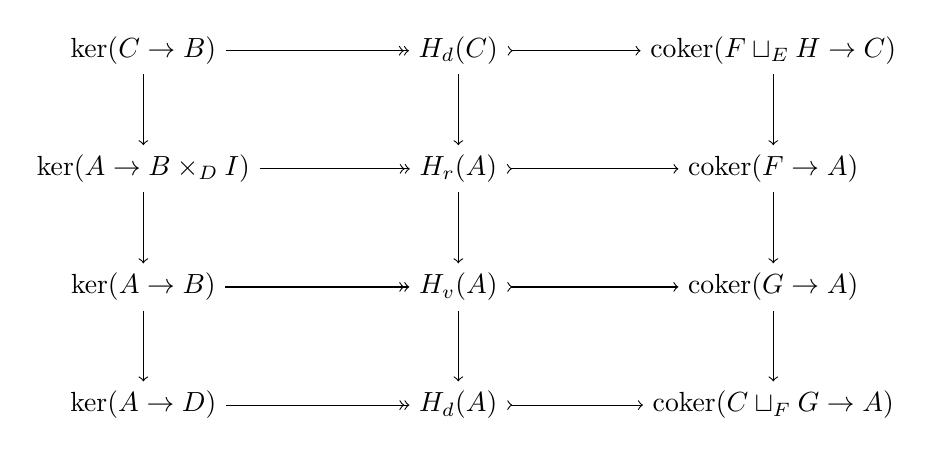
\begin{tikzpicture}
                \node (ker1) at (-4,2.25) {\(\mathrm{ker} (C \to B)\)}; \node (H1) at (0,2.25) {\(H_d (C)\)}; \node (coker1) at (4,2.25) {\(\mathrm{coker} (F \sqcup_E H \to C)\)};
                \node (ker2) at (-4,0.75) {\(\mathrm{ker} (A \to B \times_D I)\)}; \node (H2) at (0,0.75) {\(H_r (A)\)}; \node (coker2) at (4,0.75) {\(\mathrm{coker} (F \to A)\)};
                \node (ker3) at (-4,-0.75) {\(\mathrm{ker} (A \to B)\)}; \node (H3) at (0,-0.75) {\(H_v (A)\)}; \node (coker3) at (4,-0.75) {\(\mathrm{coker} (G \to A)\)};
                \node (ker4) at (-4,-2.25) {\(\mathrm{ker} (A \to D)\)}; \node (H4) at (0,-2.25) {\(H_d (A)\)}; \node (coker4) at (4,-2.25) {\(\mathrm{coker} (C \sqcup_F G \to A)\)};

                \draw[->>] (ker1) to (H1); \draw[>->] (H1) to (coker1);
                \draw[->>] (ker2) to (H2); \draw[>->] (H2) to (coker2);
                \draw[->>] (ker3) to (H3); \draw[>->] (H3) to (coker3);
                \draw[->>] (ker4) to (H4); \draw[>->] (H4) to (coker4);
                \draw[->] (ker1) to (ker2); \draw[->] (H1) to (H2); \draw[->] (coker1) to (coker2);
                \draw[->] (ker2) to (ker3); \draw[->] (H2) to (H3); \draw[->] (coker2) to (coker3);
                \draw[->] (ker3) to (ker4); \draw[->] (H3) to (H4); \draw[->] (coker3) to (coker4);
            \end{tikzpicture}
        \end{center}

        给出以下图表:

        \begin{center}
            \begin{tikzpicture}
                \node (hva) at (0,3) {\(H_v(A)\)};
                \node (ker1) at (-2,1.5) {\(\mathrm{ker} (A \to B)\)};
                \node (coker1) at (2,1.5) {\(\mathrm{coker} (G \to A)\)};
                \node (ker2) at (-4,0) {\(\mathrm{ker} (C \to B)\)};
                \node (A) at (0,0) {\(A\)};
                \node (coker2) at (4,0) {\(\mathrm{coker} (C \sqcup_F G \to A)\)};
                \node (C) at (-2,-1.5) {\(C\)};
                \node (coker) at (2,-1.5) {\(\mathrm{coker} (C \to A)\)};

                \draw[->>] (ker1) to (hva); \draw[>->] (hva) to (coker1);
                \draw[>->] (ker1) to (A); \draw[->>] (A) to (coker1);
                \draw[->] (ker2) to (ker1); \draw[->] (coker1) to (coker2);
                \draw[>->] (ker2) to (C); \draw[->>] (coker) to (coker2);
                \draw[->] (C) to (A); \draw[->] (A) to (coker);

                \node (pushout) at (2,0) {\(\boxplus\)};
                \node (pullback) at (-2,0) {\(\Box\)};
            \end{tikzpicture}
        \end{center}

        为了运用 \ref{lemma:exact sequence's pullback and pushout}, 需证明上方四边形为拉回推出, 有 \(H_v(A) = \mathrm{ker} (\mathrm{coker} (G \to A) \to \mathrm{coker} (H_v (A) \to \mathrm{coker} (G \to A)))\),
        \ref{lemma:ker of combination is a pullback} 给出 \(H_v (A) \times_{\mathrm{coker} (G \to A)} A = \mathrm{ker} (A \to \mathrm{coker} (H_v(A) \to \mathrm{coker} (G \to A)))\), 运用 \ref{lemma:definition of homology in terms of cokernels and kernels},
        便得到上方图表为拉回, 故给出正合列 \(\mathrm{ker} (C \to B) \to H_v (A) \to \mathrm{coker} (C \sqcup_F G \to A)\), 依赖单满性知 \(H_d (C) \to H_v (A) \to H_d (A)\) 亦正合.

        \(H_d (A)\) 处绘出图表如下:

        \begin{center}
            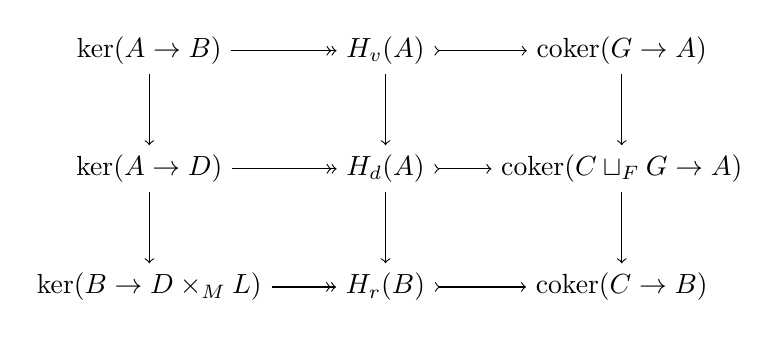
\begin{tikzpicture}
                \node (ker1) at (-3,1.5) {\(\mathrm{ker} (A \to B)\)}; \node (H1) at (0,1.5) {\(H_v (A)\)}; \node (coker1) at (3,1.5) {\(\mathrm{coker} (G \to A)\)};
                \node (ker2) at (-3,0) {\(\mathrm{ker} (A \to D)\)}; \node (H2) at (0,0) {\(H_d (A)\)}; \node (coker2) at (3,0) {\(\mathrm{coker} (C \sqcup_F G \to A)\)};
                \node (ker3) at (-3,-1.5) {\(\mathrm{ker} (B \to D \times_M L)\)}; \node (H3) at (0,-1.5) {\(H_r (B)\)}; \node (coker3) at (3,-1.5) {\(\mathrm{coker} (C \to B)\)};

                \draw[->>] (ker1) to (H1); \draw[>->] (H1) to (coker1);
                \draw[->>] (ker2) to (H2); \draw[>->] (H2) to (coker2);
                \draw[->>] (ker3) to (H3); \draw[>->] (H3) to (coker3);
                \draw[->] (ker1) to (ker2); \draw[->] (H1) to (H2); \draw[->] (coker1) to (coker2);
                \draw[->] (ker2) to (ker3); \draw[->] (H2) to (H3); \draw[->] (coker2) to (coker3);
            \end{tikzpicture}
        \end{center}

        利用 \ref{lemma:universal property of exactness symmetric} 验证正合列 \(\mathrm{ker} (A \to B) \to \mathrm{coker} (C \sqcup_F G \to A) \to \mathrm{coker} (C \to B)\),
        注意到 \(\mathrm{coker} (C \to B) = \mathrm{coker} (C \sqcup_F G \to B) = \mathrm{coker} (C \sqcup_F G \to A) \sqcup_A B\).

        \begin{center}
            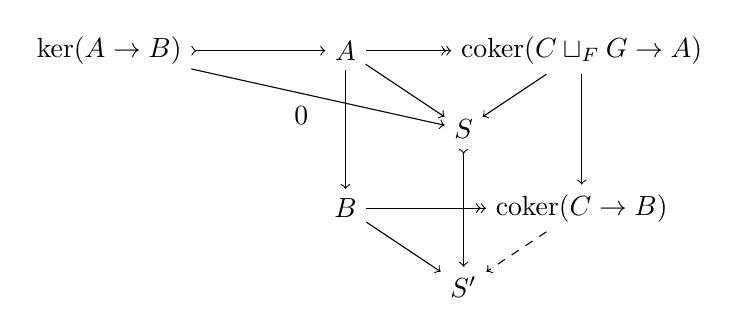
\begin{tikzpicture}
                \node (ker) at (-3,1) {\(\mathrm{ker} (A \to B)\)};
                \node (A) at (0,1) {\(A\)};
                \node (B) at (0,-1) {\(B\)};
                \node (coker1) at (3,1) {\(\mathrm{coker} (C \sqcup_F G \to A)\)};
                \node (coker2) at (3,-1) {\(\mathrm{coker} (C \to B)\)};
                \node (S) at (1.5,0) {\(S\)};
                \node (Sp) at (1.5,-2) {\(S^\prime\)};

                \draw[>->] (ker) to (A); \draw[->>] (B) to (coker2); \draw[->>] (A) to (coker1); \draw[->] (A) to (B); \draw[->] (coker1) to (coker2);
                \draw[->] (coker1) to (S); \draw[->] (A) to (S); \draw[>->] (S) to (Sp); \draw[->] (B) to (Sp); \draw[->,dashed] (coker2) to (Sp); \draw[->] (ker) to node[below left] {\(0\)} (S);
            \end{tikzpicture}
        \end{center}

        于是有交换图表:

        \begin{center}
            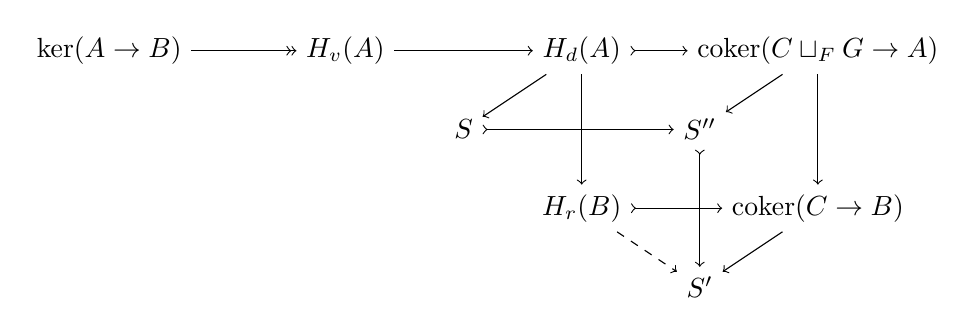
\begin{tikzpicture}
                \node (ker) at (-4.5,1) {\(\mathrm{ker} (A \to B)\)};
                \node (hva) at (-1.5,1) {\(H_v (A)\)};
                \node (hda) at (1.5,1) {\(H_d (A)\)};
                \node (coker1) at (4.5,1) {\(\mathrm{coker} (C \sqcup_F G \to A)\)};
                \node (hrb) at (1.5,-1) {\(H_r (B)\)};
                \node (coker2) at (4.5,-1) {\(\mathrm{coker} (C \to B)\)};
                \node (S) at (0,0) {\(S\)};
                \node (Sp) at (3,-2) {\(S^\prime\)};
                \node (p) at (3,0) {\(S^{\prime \prime}\)};

                \draw[->>] (ker) to (hva); \draw[->] (hva) to (hda); \draw[>->] (hda) to (coker1); \draw[->] (coker1) to (coker2); \draw[->] (hda) to (hrb); \draw[>->] (hrb) to (coker2);
                \draw[->] (hda) to (S); \draw[>->] (S) to (p); \draw[->] (coker1) to (p); \draw[->] (coker2) to (Sp); \draw[>->] (p) to (Sp); 
                \draw[->,dashed] (hrb) to (Sp);
            \end{tikzpicture}
        \end{center}

        再利用 \ref{lemma:universal property of exactness symmetric} 即得 \(H_d(A)\) 处正合. \(H_r (B)\) 处绘出交换图表如下:

        \begin{center}
            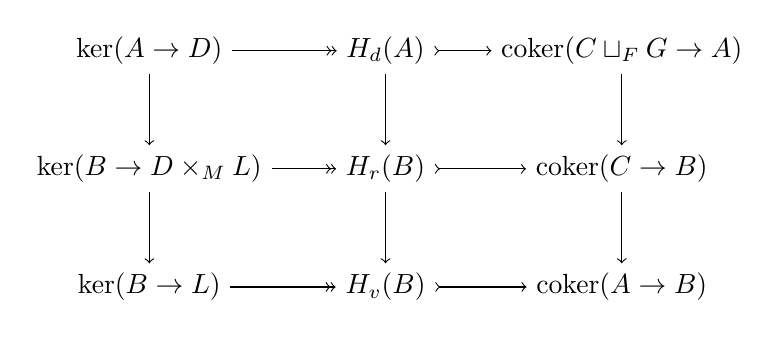
\begin{tikzpicture}
                \node (ker1) at (-3,1.5) {\(\mathrm{ker} (A \to D)\)}; \node (H1) at (0,1.5) {\(H_d (A)\)}; \node (coker1) at (3,1.5) {\(\mathrm{coker} (C \sqcup_F G \to A)\)};
                \node (ker2) at (-3,0) {\(\mathrm{ker} (B \to D \times_M L)\)}; \node (H2) at (0,0) {\(H_r (B)\)}; \node (coker2) at (3,0) {\(\mathrm{coker} (C \to B)\)};
                \node (ker3) at (-3,-1.5) {\(\mathrm{ker} (B \to L)\)}; \node (H3) at (0,-1.5) {\(H_v (B)\)}; \node (coker3) at (3,-1.5) {\(\mathrm{coker} (A \to B)\)};

                \draw[->>] (ker1) to (H1); \draw[>->] (H1) to (coker1);
                \draw[->>] (ker2) to (H2); \draw[>->] (H2) to (coker2);
                \draw[->>] (ker3) to (H3); \draw[>->] (H3) to (coker3);
                \draw[->] (ker1) to (ker2); \draw[->] (H1) to (H2); \draw[->] (coker1) to (coker2);
                \draw[->] (ker2) to (ker3); \draw[->] (H2) to (H3); \draw[->] (coker2) to (coker3);
            \end{tikzpicture}
        \end{center}

        注意到有拉回 \(\mathrm{ker} (A \to D) = \mathrm{ker} (A \to D \times_M L) = \mathrm{ker} (B \to D \times_M L) \times_B A\), 
        利用 \ref{lemma:universal property of exactness} 验证正合列 \(\mathrm{ker} (A \to D) \to \mathrm{ker} (B \to D \times_M L) \to \mathrm{coker} (A \to B)\) 如下:

        \begin{center}
            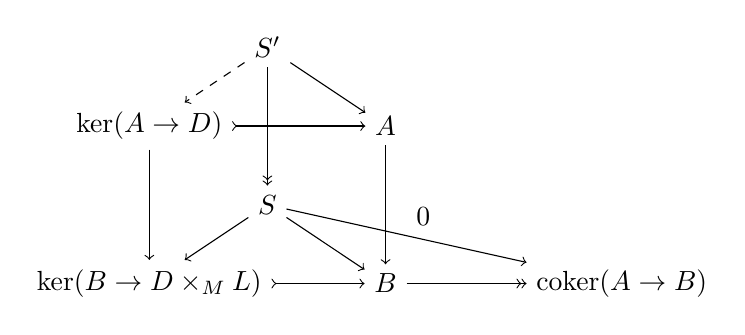
\begin{tikzpicture}
                \node (ker1) at (-3,1) {\(\mathrm{ker} (A \to D)\)};
                \node (A) at (0,1) {\(A\)};
                \node (ker2) at (-3,-1) {\(\mathrm{ker} (B \to D \times_M L)\)};
                \node (B) at (0,-1) {\(B\)};
                \node (coker) at (3,-1) {\(\mathrm{coker} (A \to B)\)};
                \node (S) at (-1.5,0) {\(S\)};
                \node (Sp) at (-1.5,2) {\(S^\prime\)};

                \draw[>->] (ker1) to (A); \draw[>->] (ker2) to (B); \draw[->] (A) to (B); \draw[->>] (B) to (coker); \draw[->] (ker1) to (ker2);
                \draw[->] (S) to (ker2); \draw[->] (S) to (B); \draw[->>] (Sp) to (S); \draw[->] (Sp) to (A); \draw[->,dashed] (Sp) to (ker1); \draw[->] (S) to node[above right] {\(0\)} (coker);
            \end{tikzpicture}
        \end{center}

        同理, 任给 \(S \to H_r (B)\), 立得图表如下, 其中 \(S^{\prime \prime}\) 为满态射的拉回:

        \begin{center}
            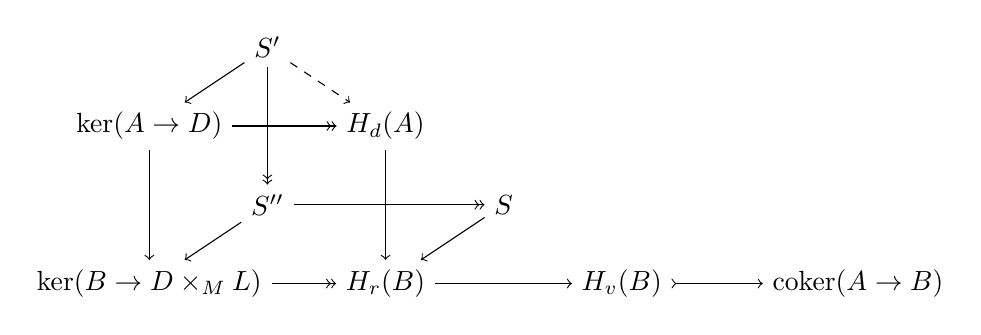
\begin{tikzpicture}
                \node (ker1) at (-4.5,1) {\(\mathrm{ker} (A \to D)\)};
                \node (ker2) at (-4.5,-1) {\(\mathrm{ker} (B \to D \times_M L)\)};
                \node (hda) at (-1.5,1) {\(H_d (A)\)};
                \node (hrb) at (-1.5,-1) {\(H_r (B)\)};
                \node (hhb) at (1.5,-1) {\(H_v (B)\)};
                \node (coker) at (4.5,-1) {\(\mathrm{coker} (A \to B)\)}; 
                \node (S) at (0,0) {\(S\)};
                \node (Sp) at (-3,2) {\(S^\prime\)};
                \node (p) at (-3,0) {\(S^{\prime \prime}\)};

                \draw[->>] (ker1) to (hda); \draw[->>] (ker2) to (hrb); \draw[->] (hda) to (hrb); \draw[->] (hrb) to (hhb); \draw[>->] (hhb) to (coker);
                \draw[->] (ker1) to (ker2); \draw[->>] (Sp) to (p); \draw[->>] (p) to (S); \draw[->] (S) to (hrb); \draw[->] (p) to (ker2); \draw[->] (Sp) to (ker1);
                \draw[->,dashed] (Sp) to (hda);
            \end{tikzpicture}
        \end{center}

        利用 \ref{lemma:universal property of exactness} 证明正合性质. 最后, \(H_v (B)\) 处绘出图表如下:

        \begin{center}
            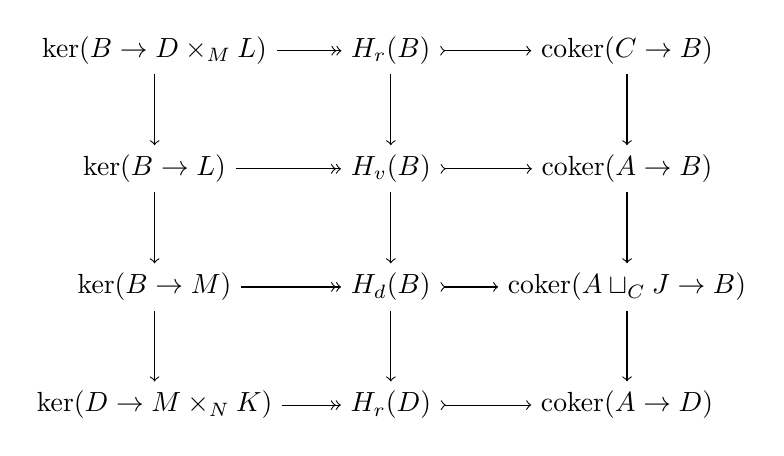
\begin{tikzpicture}
                \node (ker1) at (-3,2.25) {\(\mathrm{ker} (B \to D \times_M L)\)}; \node (H1) at (0,2.25) {\(H_r (B)\)}; \node (coker1) at (3,2.25) {\(\mathrm{coker} (C \to B)\)};
                \node (ker2) at (-3,.75) {\(\mathrm{ker} (B \to L)\)}; \node (H2) at (0,.75) {\(H_v (B)\)}; \node (coker2) at (3,.75) {\(\mathrm{coker} (A \to B)\)};
                \node (ker3) at (-3,-.75) {\(\mathrm{ker} (B \to M)\)}; \node (H3) at (0,-.75) {\(H_d (B)\)}; \node (coker3) at (3,-.75) {\(\mathrm{coker} (A \sqcup_C J \to B)\)};
                \node (ker4) at (-3,-2.25) {\(\mathrm{ker} (D \to M \times_N K)\)}; \node (H4) at (0,-2.25) {\(H_r (D)\)}; \node (coker4) at (3,-2.25) {\(\mathrm{coker} (A \to D)\)}; 

                \draw[->>] (ker1) to (H1); \draw[>->] (H1) to (coker1);
                \draw[->>] (ker2) to (H2); \draw[>->] (H2) to (coker2);
                \draw[->>] (ker3) to (H3); \draw[>->] (H3) to (coker3);
                \draw[->>] (ker4) to (H4); \draw[>->] (H4) to (coker4);
                \draw[->] (ker1) to (ker2); \draw[->] (H1) to (H2); \draw[->] (coker1) to (coker2);
                \draw[->] (ker2) to (ker3); \draw[->] (H2) to (H3); \draw[->] (coker2) to (coker3);
                \draw[->] (ker3) to (ker4); \draw[->] (H3) to (H4); \draw[->] (coker3) to (coker4);
            \end{tikzpicture}
        \end{center}

        同理得到图表如下:

        \begin{center}
            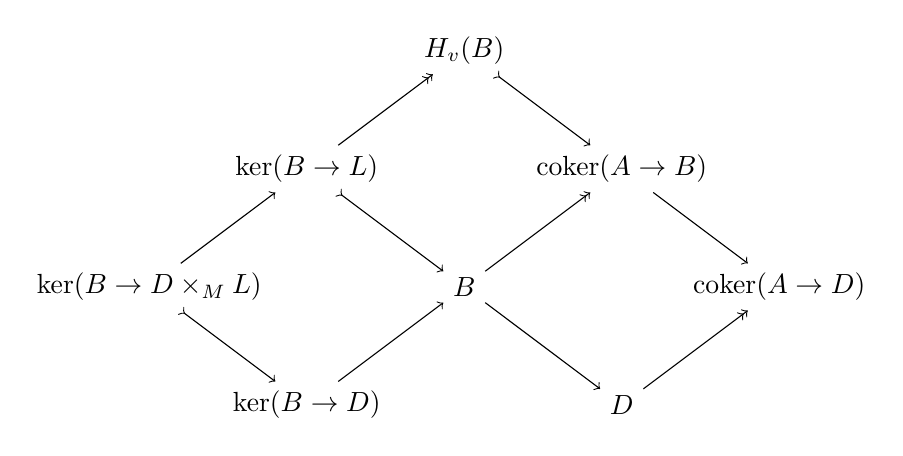
\begin{tikzpicture}
                \node (hhb) at (0,3) {\(H_v(B)\)};
                \node (ker1) at (-2,1.5) {\(\mathrm{ker} (B \to L)\)};
                \node (coker1) at (2,1.5) {\(\mathrm{coker} (A \to B)\)};
                \node (ker2) at (-4,0) {\(\mathrm{ker} (B \to D \times_M L)\)};
                \node (B) at (0,0) {\(B\)};
                \node (coker2) at (4,0) {\(\mathrm{coker} (A \to D)\)};
                \node (ker3) at (-2,-1.5) {\(\mathrm{ker} (B \to D)\)};
                \node (D) at (2,-1.5) {\(D\)};

                \draw[->>] (ker1) to (hhb); \draw[>->] (hhb) to (coker1);
                \draw[>->] (ker1) to (B); \draw[->>] (B) to (coker1);
                \draw[->] (ker2) to (ker1); \draw[->] (coker1) to (coker2);
                \draw[>->] (ker2) to (ker3); \draw[->>] (D) to (coker2);
                \draw[->] (B) to (D); \draw[->] (ker3) to (B);
            \end{tikzpicture}
        \end{center}

        同理运用 \ref{lemma:exact sequence's pullback and pushout} 与 \ref{lemma:definition of homology in terms of cokernels and kernels} 即得到正合列.
    \end{proof}
\end{lemma}

称上述图表为在 \(A \to B\) 处的蝾螈引理.

\subsubsection{蝾螈引理应用}

\begin{corollary}
    给出双复形中图表如下, 且该横行于 \(A,B\) 处正合:

    \begin{center}
        \begin{tikzpicture}
            \node (A) at (-2,0) {\(A\)};
            \node (B) at (2,0) {\(B\)};

            \draw[->] (A) to (B);
        \end{tikzpicture}
    \end{center}

    则 \(H_d (A) \to H_r (B)\) 是同构.

    \begin{proof}
        \(A \to B\) 的 \ref{lemma:salamander lemma} 给出正合列:

        \[
            0 = H_h (A) \to H_d (A) \to H_r (A) \to H_h (B) = 0
        \]

        故 \(H_d (A) = H_r (B)\).
    \end{proof}
\end{corollary}

\begin{corollary}
    给出双复形中图表如下, 则有对应的同构, 对称的, 倒转箭头方向与翻转也可得类似的同构:

    \begin{center}
        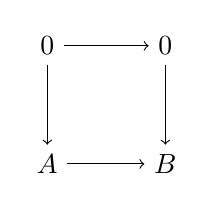
\begin{tikzpicture}
            \node (01) at (-.75,.75) {\(0\)};
            \node (02) at (.75,.75) {\(0\)};
            \node (A) at (-.75,-.75) {\(A\)};
            \node (B) at (.75,-.75) {\(B\)};

            \draw[->] (01) to (02); \draw[->] (01) to (A);
            \draw[->] (A) to (B); \draw[->] (02) to (B);
        \end{tikzpicture} 
    \end{center}
    
    \[
        \begin{matrix}
            H_r (A) = H_v (A) \\
            H_h (A) = H_d (A)
        \end{matrix}
    \]

    \begin{proof}
        \(0 \to B\) 的 \ref{lemma:salamander lemma} 给出 \(0 = H_d(0) \to H_r (B) \to H_v (B) = 0\),
        故 \(H_r (B) = 0\), \(0 \to A\) 的 \ref{lemma:salamander lemma} 给出 \(0 = H_d(0) \to H_r (A) \to H_v (A) \to H_r (B) = 0\),
        故 \(H_r (A) = H_v (A)\), \(A \to B\) 的 \ref{lemma:salamander lemma} 给出 \(0 = H_d (0) \to H_h(A) \to H_d (A) \to H_r (B) = 0\),
        故 \(H_h (A) = H_d (A)\).
    \end{proof}
\end{corollary}

\begin{lemma}[\(3 \times 3\) 引理]
    给出图表如下, 且纵列均正合, 第二, 三横行正合, 则第一横行亦正合.

    \begin{center}
        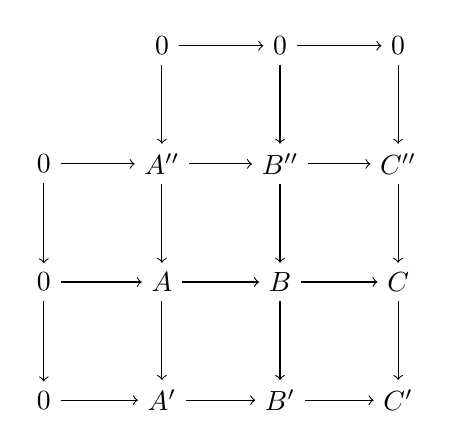
\begin{tikzpicture}
            \node (01) at (-1.5,3) {\(0\)};
            \node (02) at (0,3) {\(0\)};
            \node (03) at (1.5,3) {\(0\)};
            \node (04) at (-3,1.5) {\(0\)};
            \node (App) at (-1.5,1.5) {\(A^{\prime \prime}\)};
            \node (Bpp) at (0,1.5) {\(B^{\prime \prime}\)};
            \node (Cpp) at (1.5,1.5) {\(C^{\prime \prime}\)};
            \node (05) at (-3,0) {\(0\)};
            \node (A) at (-1.5,0) {\(A\)};
            \node (B) at (0,0) {\(B\)};
            \node (C) at (1.5,0) {\(C\)};
            \node (06) at (-3,-1.5) {\(0\)};
            \node (Ap) at (-1.5,-1.5) {\(A^\prime\)};
            \node (Bp) at (0,-1.5) {\(B^\prime\)};
            \node (Cp) at (1.5,-1.5) {\(C^\prime\)};

            \draw[->] (01) to (02); \draw[->] (02) to (03);
            \draw[->] (04) to (App); \draw[->] (App) to (Bpp); \draw[->] (Bpp) to (Cpp);
            \draw[->] (05) to (A); \draw[->] (A) to (B); \draw[->] (B) to (C);
            \draw[->] (06) to (Ap); \draw[->] (Ap) to (Bp); \draw[->] (Bp) to (Cp);
            \draw[->] (01) to (App); \draw[->] (02) to (Bpp); \draw[->] (03) to (Cpp);
            \draw[->] (04) to (05); \draw[->] (App) to (A); \draw[->] (Bpp) to (B); \draw[->] (Cpp) to (C);
            \draw[->] (05) to (06); \draw[->] (A) to (Ap); \draw[->] (B) to (Bp); \draw[->] (C) to (Cp);
        \end{tikzpicture}
    \end{center}

    \begin{proof}
        有 \(H_h (A^{\prime \prime}) = H_d (A^{\prime \prime}) = H_r (A) = H_d (0) = 0\),
        \(H_h (B^{\prime \prime}) = H_d (B^{\prime \prime}) = H_r (B) = H_d (A) = H_r (A^\prime) = H_d (0) = 0\).
    \end{proof}
\end{lemma}

\begin{corollary}
    同理, 如果扩充成下图, 使得纵列均正合且二, 三横行正合, 则第一横行亦正合.

    \begin{center}
        \begin{tikzpicture}
            \node (01) at (-1.5,3) {\(0\)};
            \node (02) at (0,3) {\(0\)};
            \node (03) at (1.5,3) {\(0\)};
            \node (04) at (-3,1.5) {\(0\)};
            \node (App) at (-1.5,1.5) {\(A^{\prime \prime}\)};
            \node (Bpp) at (0,1.5) {\(B^{\prime \prime}\)};
            \node (Cpp) at (1.5,1.5) {\(C^{\prime \prime}\)};
            \node (05) at (-3,0) {\(0\)};
            \node (A) at (-1.5,0) {\(A\)};
            \node (B) at (0,0) {\(B\)};
            \node (C) at (1.5,0) {\(C\)};
            \node (06) at (-3,-1.5) {\(0\)};
            \node (Ap) at (-1.5,-1.5) {\(A^\prime\)};
            \node (Bp) at (0,-1.5) {\(B^\prime\)};
            \node (Cp) at (1.5,-1.5) {\(C^\prime\)};
            \node (07) at (3,1.5) {\(0\)};
            \node (08) at (3,0) {\(0\)};
            \node (09) at (-1.5,-3) {\(0\)};

            \draw[->] (01) to (02); \draw[->] (02) to (03);
            \draw[->] (04) to (App); \draw[->] (App) to (Bpp); \draw[->] (Bpp) to (Cpp);
            \draw[->] (05) to (A); \draw[->] (A) to (B); \draw[->] (B) to (C);
            \draw[->] (06) to (Ap); \draw[->] (Ap) to (Bp); \draw[->] (Bp) to (Cp);
            \draw[->] (01) to (App); \draw[->] (02) to (Bpp); \draw[->] (03) to (Cpp);
            \draw[->] (04) to (05); \draw[->] (App) to (A); \draw[->] (Bpp) to (B); \draw[->] (Cpp) to (C);
            \draw[->] (05) to (06); \draw[->] (A) to (Ap); \draw[->] (B) to (Bp); \draw[->] (C) to (Cp);
            \draw[->] (Cpp) to (07); \draw[->] (C) to (08); \draw[->] (Ap) to (09); \draw[->] (07) to (08);
        \end{tikzpicture}
    \end{center}

    \begin{proof}
        同理, 有 \(H_h (C^{\prime \prime}) = H_d (C^{\prime \prime}) = H_r (C) = H_d (B) = H_r (B^\prime) = H_d (A^\prime) = H_r (0) = 0\).
    \end{proof}
\end{corollary}

\begin{lemma}[蛇引理]
    \setlabel {蛇引理}
    \label {lemma:snake lemma}
    若下述图表横行皆正合, 且 \(f_0\) 满 \(f_4\) 单.

    \begin{center}
        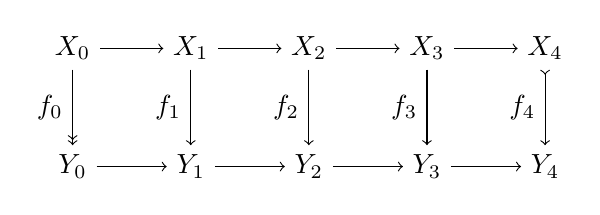
\begin{tikzpicture}
            \node (X0) at (-3,.75) {\(X_0\)};
            \node (X1) at (-1.5,.75) {\(X_1\)};
            \node (X2) at (0,.75) {\(X_2\)};
            \node (X3) at (1.5,.75) {\(X_3\)};
            \node (X4) at (3,.75) {\(X_4\)};
            \node (Y0) at (-3,-.75) {\(Y_0\)};
            \node (Y1) at (-1.5,-.75) {\(Y_1\)};
            \node (Y2) at (0,-.75) {\(Y_2\)};
            \node (Y3) at (1.5,-.75) {\(Y_3\)};
            \node (Y4) at (3,-.75) {\(Y_4\)};

            \draw[->] (X0) to (X1); \draw[->] (X1) to (X2); \draw[->] (X2) to (X3); \draw[->] (X3) to (X4);
            \draw[->] (Y0) to (Y1); \draw[->] (Y1) to (Y2); \draw[->] (Y2) to (Y3); \draw[->] (Y3) to (Y4);
            \draw[->>] (X0) to node[left] {\(f_0\)} (Y0); \draw[->] (X1) to node[left] {\(f_1\)} (Y1); \draw[->] (X2) to node[left] {\(f_2\)} (Y2); \draw[->] (X3) to node[left] {\(f_3\)} (Y3); \draw[>->] (X4) to node[left] {\(f_4\)} (Y4);
        \end{tikzpicture}
    \end{center}

    令 \(K_i = \mathrm{ker} (f_i),C_i = \mathrm{coker} (f_i)\), 则有正合列:

    \[
        K_1 \to K_2 \to K_3 \to C_1 \to C_2 \to C_3
    \]

    \begin{proof}
        嵌入双复形中得到以下图表:

        \begin{center}
            \begin{tikzpicture}
                \node (K1) at (-1.5,2.25) {\(K_1\)};
                \node (K2) at (0,2.25) {\(K_2\)};
                \node (K3) at (1.5,2.25) {\(K_3\)};
                \node (0K) at (3,2.25) {\(0\)};
                \node (X0) at (-3,.75) {\(X_0\)};
                \node (X1) at (-1.5,.75) {\(X_1\)};
                \node (X2) at (0,.75) {\(X_2\)};
                \node (X3) at (1.5,.75) {\(X_3\)};
                \node (X4) at (3,.75) {\(X_4\)};
                \node (Y0) at (-3,-.75) {\(Y_0\)};
                \node (Y1) at (-1.5,-.75) {\(Y_1\)};
                \node (Y2) at (0,-.75) {\(Y_2\)};
                \node (Y3) at (1.5,-.75) {\(Y_3\)};
                \node (Y4) at (3,-.75) {\(Y_4\)};
                \node (0C) at (-3,-2.25) {\(0\)};
                \node (C1) at (-1.5,-2.25) {\(C_1\)};
                \node (C2) at (0,-2.25) {\(C_2\)};
                \node (C3) at (1.5,-2.25) {\(C_3\)};

                \draw[->] (K1) to (K2); \draw[->] (K2) to (K3); \draw[->] (K3) to (0K);
                \draw[->] (X0) to (X1); \draw[->] (X1) to (X2); \draw[->] (X2) to (X3); \draw[->] (X3) to (X4);
                \draw[->] (Y0) to (Y1); \draw[->] (Y1) to (Y2); \draw[->] (Y2) to (Y3); \draw[->] (Y3) to (Y4);
                \draw[->] (0C) to (C1); \draw[->] (C1) to (C2); \draw[->] (C2) to (C3);
                \draw[->] (K1) to (X1); \draw[->] (K2) to (X2); \draw[->] (K3) to (X3); \draw[->] (0K) to (X4);
                \draw[->] (X0) to (Y0); \draw[->] (X1) to (Y1); \draw[->] (X2) to (Y2); \draw[->] (X3) to (Y3); \draw[->] (X4) to (Y4);
                \draw[->] (Y0) to (0C); \draw[->] (Y1) to (C1); \draw[->] (Y2) to (C2); \draw[->] (Y3) to (C3);

                \node (coker) at (4.5,.75) {\(\mathrm{coker}\)};
                \node (ker) at (-4.5,-.75) {\(\mathrm{ker}\)};

                \draw[->] (X4) to (coker); \draw[->] (ker) to (Y0);
            \end{tikzpicture}
        \end{center}

        我们构造连接态射 \(\delta : K_3 \to C_1\) 为
        
        \[
            \delta := K_3 \to \mathrm{coker} (K_2 \to K_3) = H_h (K_3) = H_h (C_1) = \mathrm{ker} (C_1 \to C_2) \to C_1
        \]

        其中 \(H_h (K_3) = H_h (C_1)\) 在上下方补 \(0\) 后基于图表正合性给出等式
        \(H_h (K_3) = H_d (K_3) = H_r (X_3) = H_d (X_2) = H_r (Y_2) = H_d (Y_1) = H_r (C_1) = H_h (C_1)\)

        只需验证 \(K_2,C_2\) 处正合性, 只需注意到等式 
        
        \[
            \begin{aligned}
                H_h (K_2) = H_d (K_2) = H_r (X_2) = H_d (X_1) = H_r (Y_1) = H_d (Y_0) = H_r (0) = 0 \\
                H_h (C_2) = H_r (C_2) = H_d (Y_2) = H_r (Y_3) = H_d (X_3) = H_r (X_4) = H_d (0) = 0
            \end{aligned}
        \]
    \end{proof}
\end{lemma}

\begin{lemma}[五项引理]
    给出横行正合的交换图表如下:

    \begin{center}
        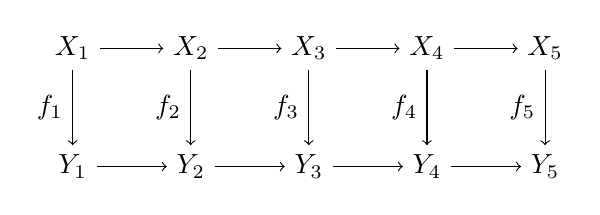
\begin{tikzpicture}
            \node (X1) at (-3,.75) {\(X_1\)};
            \node (X2) at (-1.5,.75) {\(X_2\)};
            \node (X3) at (0,.75) {\(X_3\)};
            \node (X4) at (1.5,.75) {\(X_4\)};
            \node (X5) at (3,.75) {\(X_5\)};
            \node (Y1) at (-3,-.75) {\(Y_1\)};
            \node (Y2) at (-1.5,-.75) {\(Y_2\)};
            \node (Y3) at (0,-.75) {\(Y_3\)};
            \node (Y4) at (1.5,-.75) {\(Y_4\)};
            \node (Y5) at (3,-.75) {\(Y_5\)};

            \draw[->] (X1) to (X2); \draw[->] (X2) to (X3); \draw[->] (X3) to (X4); \draw[->] (X4) to (X5);
            \draw[->] (Y1) to (Y2); \draw[->] (Y2) to (Y3); \draw[->] (Y3) to (Y4); \draw[->] (Y4) to (Y5);
            \draw[->] (X1) to node[left] {\(f_1\)} (Y1); \draw[->] (X2) to node[left] {\(f_2\)} (Y2); \draw[->] (X3) to node[left] {\(f_3\)} (Y3); \draw[->] (X4) to node[left] {\(f_4\)} (Y4); \draw[->] (X5) to node[left] {\(f_5\)} (Y5);
        \end{tikzpicture}
    \end{center}

    \begin{enumerate}
        \item 若 \(f_1\) 满, \(f_2,f_4\) 单, 则 \(f_3\) 亦单.
        \item 若 \(f_5\) 单, \(f_4,f_2\) 满, 则 \(f_3\) 亦满.
        \item 若 \(f_1\) 满, \(f_5\) 单, \(f_2,f_4\) 为同构, 则 \(f_3\) 亦为同构.
    \end{enumerate}

    \begin{proof}
        显然第三条是前两条的推论, 我们证明第一条, 注意到 \(I_X := \mathrm{im} (X_3 \to X_4) \to X_4 \to Y_4 = I_X \to I_Y := \mathrm{im} (Y_3 \to Y_4) \to Y_4\) 单, 故 \(I_X \to I_Y\) 亦单,
        对以下图表运用 \ref{lemma:snake lemma} 即可:

        \begin{center}
            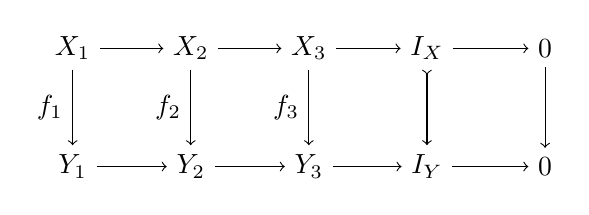
\begin{tikzpicture}
                \node (X1) at (-3,.75) {\(X_1\)};
                \node (X2) at (-1.5,.75) {\(X_2\)};
                \node (X3) at (0,.75) {\(X_3\)};
                \node (X4) at (1.5,.75) {\(I_X\)};
                \node (X5) at (3,.75) {\(0\)};
                \node (Y1) at (-3,-.75) {\(Y_1\)};
                \node (Y2) at (-1.5,-.75) {\(Y_2\)};
                \node (Y3) at (0,-.75) {\(Y_3\)};
                \node (Y4) at (1.5,-.75) {\(I_Y\)};
                \node (Y5) at (3,-.75) {\(0\)};

                \draw[->] (X1) to (X2); \draw[->] (X2) to (X3); \draw[->] (X3) to (X4); \draw[->] (X4) to (X5);
                \draw[->] (Y1) to (Y2); \draw[->] (Y2) to (Y3); \draw[->] (Y3) to (Y4); \draw[->] (Y4) to (Y5);
                \draw[->] (X1) to node[left] {\(f_1\)} (Y1); \draw[->] (X2) to node[left] {\(f_2\)} (Y2); \draw[->] (X3) to node[left] {\(f_3\)} (Y3); \draw[>->] (X4) to (Y4); \draw[->] (X5) to (Y5);
            \end{tikzpicture}
        \end{center}
    \end{proof}
\end{lemma}

\begin{lemma}[Noether 第二同构定理]
    给出单态射 \(\sigma : X \to Y, \psi : Y \to Z\), 则 \(Z/Y \cong (Z/X) / (Y/X)\), 其中 \(/\) 表示 \(\mathrm{coker}\).

    \begin{center}
        \begin{tikzpicture}
            \node (01) at (-1.5,3) {\(0\)};
            \node (02) at (0,3) {\(0\)};
            \node (X1) at (-1.5,1.5) {\(X\)};
            \node (X2) at (0,1.5) {\(X\)};
            \node (03) at (-3,0) {\(0\)};
            \node (Y) at (-1.5,0) {\(Y\)};
            \node (Z) at (0,0) {\(Z\)};
            \node (ZY) at (2,0) {\(Z / Y\)};
            \node (04) at (4,0) {\(0\)};
            \node (05) at (-3,-1.5) {\(0\)};
            \node (YX) at (-1.5,-1.5) {\(Y / X\)};
            \node (ZX) at (0,-1.5) {\(Z / X\)};
            \node (ZYX) at (2,-1.5) {\((Z / X) / (Y / X)\)};
            \node (06) at (4,-1.5) {\(0\)};
            \node (07) at (-1.5,-3) {\(0\)};
            \node (08) at (0,-3) {\(0\)};

            \draw[->] (01) to (02); \draw[->] (X1) to (X2); \draw[->] (01) to (X1); \draw[->] (02) to (X2); \draw[->] (X1) to (Y); \draw[->] (X2) to (Z); 
            \draw[->] (03) to (Y); \draw[->] (Y) to (Z); \draw[->] (Z) to (ZY); \draw[->] (ZY) to (04); \draw[->] (05) to (YX); \draw[->] (YX) to (ZX); \draw[->] (ZX) to (ZYX); \draw[->] (ZYX) to (06);
            \draw[->] (03) to (05); \draw[->] (Y) to (YX); \draw[->] (Z) to (ZX); \draw[->] (ZY) to (ZYX); \draw[->] (04) to (06);
            \draw[->] (07) to (08); \draw[->] (YX) to (07); \draw[->] (ZX) to (08);
        \end{tikzpicture}
    \end{center}

    \begin{proof}
        对左边两列运用 \ref{lemma:snake lemma} 即可.
    \end{proof}
\end{lemma}

\begin{lemma}
    双复形所有纵列正合, 给出子图如下:

    \begin{center}
        \begin{tikzpicture}
            \node (A) at (-.75,2.25) {\(A\)};
            \node (B) at (.75,2.25) {\(B\)};
            \node (C) at (2.25,2.25) {\(C\)};
            \node (D) at (3.75,2.25) {\(D\)};
            \node (E) at (-2.25,.75) {\(E\)};
            \node (F) at (-.75,.75) {\(F\)};
            \node (G) at (.75,.75) {\(G\)};
            \node (H) at (2.25,.75) {\(H\)};
            \node (I) at (-3.75,-.75) {\(I\)};
            \node (J) at (-2.25,-.75) {\(J\)};
            \node (K) at (-.75,-.75) {\(K\)};
            \node (L) at (.75,-.75) {\(L\)};
            \node (M) at (-3.75,-2.25) {\(M\)};
            \node (N) at (-2.25,-2.25) {\(N\)};
            \node (O) at (-.75,-2.25) {\(O\)};
            \node (P) at (.75,-2.25) {\(P\)};

            \draw[->] (A) to (B); \draw[->] (B) to (C); \draw[->] (C) to (D);
            \draw[->] (E) to (F); \draw[->] (F) to (G); \draw[->] (G) to (H);
            \draw[->] (I) to (J); \draw[->] (J) to (K); \draw[->] (K) to (L);
            \draw[->] (M) to (N); \draw[->] (N) to (O); \draw[->] (O) to (P);
            \draw[->] (A) to (F); \draw[->] (B) to (G); \draw[->] (C) to (H);
            \draw[->] (E) to (J); \draw[->] (F) to (K); \draw[->] (G) to (L);
            \draw[->] (I) to (M); \draw[->] (J) to (N); \draw[->] (K) to (O); \draw[->] (L) to (P);
        \end{tikzpicture}
    \end{center}

    诱导出以下横行均正合的交换图表:

    \begin{center}
        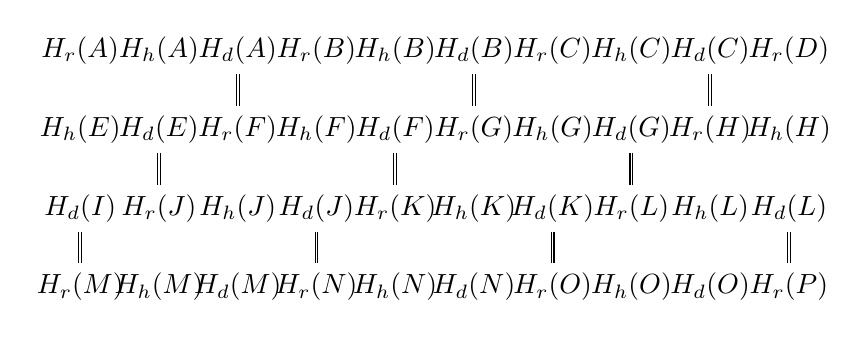
\begin{tikzpicture}
            \node (Ar) at (-4.5,1.5) {\(H_r (A)\)};
            \node (Ah) at (-3.5,1.5) {\(H_h (A)\)};
            \node (Ad) at (-2.5,1.5) {\(H_d (A)\)};
            \node (Br) at (-1.5,1.5) {\(H_r (B)\)};
            \node (Bh) at (-.5,1.5) {\(H_h (B)\)};
            \node (Bd) at (.5,1.5) {\(H_d (B)\)};
            \node (Cr) at (1.5,1.5) {\(H_r (C)\)};
            \node (Ch) at (2.5,1.5) {\(H_h (C)\)};
            \node (Cd) at (3.5,1.5) {\(H_d (C)\)};
            \node (Dr) at (4.5,1.5) {\(H_r (D)\)};

            \node (Eh) at (-4.5,.5) {\(H_h (E)\)};
            \node (Ed) at (-3.5,.5) {\(H_d (E)\)};
            \node (Fr) at (-2.5,.5) {\(H_r (F)\)};
            \node (Fh) at (-1.5,.5) {\(H_h (F)\)};
            \node (Fd) at (-.5,.5) {\(H_d (F)\)};
            \node (Gr) at (.5,.5) {\(H_r (G)\)};
            \node (Gh) at (1.5,.5) {\(H_h (G)\)};
            \node (Gd) at (2.5,.5) {\(H_d (G)\)};
            \node (Hr) at (3.5,.5) {\(H_r (H)\)};
            \node (Hh) at (4.5,.5) {\(H_h (H)\)};

            \node (Id) at (-4.5,-.5) {\(H_d (I)\)};
            \node (Jr) at (-3.5,-.5) {\(H_r (J)\)};
            \node (Jh) at (-2.5,-.5) {\(H_h (J)\)};
            \node (Jd) at (-1.5,-.5) {\(H_d (J)\)};
            \node (Kr) at (-.5,-.5) {\(H_r (K)\)};
            \node (Kh) at (.5,-.5) {\(H_h (K)\)};
            \node (Kd) at (1.5,-.5) {\(H_d (K)\)};
            \node (Lr) at (2.5,-.5) {\(H_r (L)\)};
            \node (Lh) at (3.5,-.5) {\(H_h (L)\)};
            \node (Ld) at (4.5,-.5) {\(H_d (L)\)};

            \node (Mr) at (-4.5,-1.5) {\(H_r (M)\)};
            \node (Mh) at (-3.5,-1.5) {\(H_h (M)\)};
            \node (Md) at (-2.5,-1.5) {\(H_d (M)\)};
            \node (Nr) at (-1.5,-1.5) {\(H_r (N)\)};
            \node (Nh) at (-.5,-1.5) {\(H_h (N)\)};
            \node (Nd) at (.5,-1.5) {\(H_d (N)\)};
            \node (Or) at (1.5,-1.5) {\(H_r (O)\)};
            \node (Oh) at (2.5,-1.5) {\(H_h (O)\)};
            \node (Od) at (3.5,-1.5) {\(H_d (O)\)};
            \node (Pr) at (4.5,-1.5) {\(H_r (P)\)};

            \draw[double] (Ad) to (Fr); \draw[double] (Bd) to (Gr); \draw[double] (Cd) to (Hr);
            \draw[double] (Ed) to (Jr); \draw[double] (Fd) to (Kr); \draw[double] (Gd) to (Lr);
            \draw[double] (Id) to (Mr); \draw[double] (Jd) to (Nr); \draw[double] (Kd) to (Or); \draw[double] (Ld) to (Pr);
        \end{tikzpicture}
    \end{center}

    \begin{proof}
        对横行运用 \ref{lemma:salamander lemma}, 并且运用正合列诱导出的 \(H_d = H_r\) 即可.
    \end{proof}
\end{lemma}

\subsection{复形, 解消}

\subsubsection{同伦}

\begin{definition}[平移函子]
    \label {definition:shift functor}
    对复形 \(X \in \mathbf{C} (\mathcal{A})\) 定义复形 \(X[n]\) 如下:

    \[
        {(X[n])}^k := X^{k + n}, d_{X[n]}^{k} := {(-1)}^n d_X^{k+n}
    \]

    显见其为加性函子且有

    \begin{enumerate}
        \item \([0] = \mathrm{id}_{\mathbf{C} (\mathcal{A})}\)
        \item \([n] \circ [m] = [n + m]\)
        \item 有复形间的态射 \(d_X : X \to X[1]\)
    \end{enumerate}
\end{definition}

\begin{definition}[\(\mathrm{Hom}\) - 复形]
    给出 \(X,Y \in \mathbf{C} (\mathcal{A})\), 定义

    \[
        \mathrm{Hom}^n (X,Y) := \prod_{k \in \mathbb{Z}} \mathrm{Hom} (X^k,Y^{k+n})
    \]

    显见态射合成给出如下同态:

    \[
        \mathrm{Hom}^m (X,Y) \times \mathrm{Hom}^n (Y,Z) \to \mathrm{Hom}^{m+n} (X,Z)
    \]

    有 \(d_X \in \mathrm{Hom}^1 (X,X),d_Y \in \mathrm{Hom}^1 (Y,Y)\) 定义复形 \(\mathrm{Hom}^n (X,Y)\) 的微分:

    \[
        d^n_{\mathrm{Hom}^\bullet (X,Y)} : \mathrm{Hom}^n (X,Y) \to \mathrm{Hom}^{n+1} (X,Y), f \mapsto d_Y \circ f - (-1)^n f \circ d_X
    \]
\end{definition}

\newpage

\subsection{三角范畴, 导出范畴}

\subsubsection{三角范畴}

\begin{definition}[平移]
    一个带平移的范畴定义为 \((\mathcal{D},T)\) 使得 \(T\) 是 \(\mathcal{D} \to \mathcal{D}\) 的等价,
    称 \(T\) 是平移函子.
\end{definition}

\begin{corollary}
    上述提及的 \ref{definition:graded object} 显然是带平移的范畴.
\end{corollary}

\begin{definition}
    带平移范畴间的函子是与平移相容的一个函子 \(F : \mathcal{D} \to \mathcal{D}^\prime\) 也即 \(F \circ T \cong T^\prime \circ F\).
\end{definition}

\begin{definition}
    带平移范畴间函子的自然变换定义为与平移相容的自然变换.

    \begin{center}
        \begin{tikzpicture}
            \node (FT) at (-1.5,.75) {\(F T\)};
            \node (FpT) at (1.5,.75) {\(F^\prime T\)};
            \node (TF) at (-1.5,-.75) {\(T^\prime F\)};
            \node (TFp) at (1.5,-.75) {\(T^\prime F^\prime\)};

            \draw[->] (FT) to (FpT); \draw[->] (FT) to (TF); \draw[->] (FpT) to (TFp); \draw[->] (TF) to (TFp); 
        \end{tikzpicture}
    \end{center}
\end{definition}

\begin{definition}
    一个带平移范畴 \((\mathcal{D},T)\) 中的三角指以下图表:

    \begin{center}
        \begin{tikzpicture}
            \node (X) at (-4.5,0) {\(X\)};
            \node (Y) at (-1.5,0) {\(Y\)};
            \node (Z) at (1.5,0) {\(Z\)};
            \node (TX) at (4.5,0) {\(T X\)};

            \draw[->] (X) to (Y); \draw[->] (Y) to (Z); \draw[->] (Z) to (TX);
        \end{tikzpicture}
    \end{center}

    三角间的同态是交换图表:

    \begin{center}
        \begin{tikzpicture}
            \node (X) at (-4.5,0) {\(X\)};
            \node (Y) at (-1.5,0) {\(Y\)};
            \node (Z) at (1.5,0) {\(Z\)};
            \node (TX) at (4.5,0) {\(T X\)};
            \node (Xp) at (-4.5,-1.5) {\(X^\prime\)};
            \node (Yp) at (-1.5,-1.5) {\(Y^\prime\)};
            \node (Zp) at (1.5,-1.5) {\(Z^\prime\)};
            \node (TXp) at (4.5,-1.5) {\(T X^\prime\)};

            \draw[->] (X) to (Y); \draw[->] (Y) to (Z); \draw[->] (Z) to (TX);
            \draw[->] (Xp) to (Yp); \draw[->] (Yp) to (Zp); \draw[->] (Zp) to (TXp);
            \draw[->] (X) to node[left] {\(\alpha\)} (Xp); \draw[->] (Y) to (Yp); \draw[->] (Z) to (Zp); \draw[->] (TX) to node[left] {\(T \alpha\)} (TXp);
        \end{tikzpicture}
    \end{center}
\end{definition}

\begin{definition}[三角范畴]
    \label {definition:triangulated category}
    一个带平移的加性范畴 \((\mathcal{D},T)\) 是三角范畴, 如果有一族三角 \(\mathfrak{T}\) 称好三角满足以下公理:

    \begin{enumerate}
        \item 若一个三角形同构于 \(\mathfrak{T}\) 中的某个三角, 则其在 \(\mathfrak{T}\) 中.
        \item 任意对象 \(X\) 诱导出的 \(X \to X \to 0 \to T X\) 为 \(\mathfrak{T}\) 中的三角.
        \item 任意态射 \(f : X \to Y\) 均可诱导出某个 \(X \to Y \to Z \to T X\) 为 \(\mathfrak{T}\) 中的三角.
        \item 给出三角 \(X \xrightarrow{f} Y \xrightarrow{g} Z \xrightarrow{h} T X\) 在 \(\mathfrak{T}\) 中, 则 \(Y \xrightarrow{-g} Z \xrightarrow{-h} T X \xrightarrow{-T f} T Y\) 也在 \(\mathfrak{T}\) 中.
        \item 给出 \(\mathfrak{T}\) 中两个三角, 且左侧矩形交换, 则存在 \(\gamma\) 使下图交换:
            \begin{center}
                \begin{tikzpicture}
                    \node (X) at (-4.5,0) {\(X\)};
                    \node (Y) at (-1.5,0) {\(Y\)};
                    \node (Z) at (1.5,0) {\(Z\)};
                    \node (TX) at (4.5,0) {\(T X\)};
                    \node (Xp) at (-4.5,-1.5) {\(X^\prime\)};
                    \node (Yp) at (-1.5,-1.5) {\(Y^\prime\)};
                    \node (Zp) at (1.5,-1.5) {\(Z^\prime\)};
                    \node (TXp) at (4.5,-1.5) {\(T X^\prime\)};

                    \draw[->] (X) to (Y); \draw[->] (Y) to (Z); \draw[->] (Z) to (TX);
                    \draw[->] (Xp) to (Yp); \draw[->] (Yp) to (Zp); \draw[->] (Zp) to (TXp);
                    \draw[->] (X) to node[left] {\(\alpha\)} (Xp); \draw[->] (Y) to node[left] {\(\beta\)} (Yp); \draw[->,dashed] (Z) to node[left] {\(\gamma\)} (Zp); \draw[->] (TX) to node[left] {\(T \alpha\)} (TXp);
                \end{tikzpicture}
            \end{center}
        \item 满足八面体图表交换, 即给出 \(\mathfrak{T}\) 中三角如下:
            \[
                \begin{aligned}
                    X & \xrightarrow{f} & Y & \xrightarrow{g} & Z^\prime & \to & T X \\
                    Y & \xrightarrow{g} & Z & \xrightarrow{k} & X^\prime & \to & T Y \\
                    X & \xrightarrow{gf} & Z & \xrightarrow{h} & Y^\prime & \to & T X
                \end{aligned}
            \]

            必然有 \(\mathfrak{T}\) 中三角 \(Z^\prime \xrightarrow{u} Y^\prime \xrightarrow{v} X^\prime \xrightarrow{w} T Z^\prime\) 使得以下图表交换:

            \begin{center}
                \begin{tikzpicture}
                    \node (X1) at (-4.5,2.25) {\(X\)};
                    \node (Y1) at (-1.5,2.25) {\(Y\)};
                    \node (Zp1) at (1.5,2.25) {\(Z^\prime\)};
                    \node (TX1) at (4.5,2.25) {\(T X\)};
                    \node (X2) at (-4.5,.75) {\(X\)};
                    \node (Z1) at (-1.5,.75) {\(Z\)};
                    \node (Yp1) at (1.5,.75) {\(Y^\prime\)};
                    \node (TX2) at (4.5,.75) {\(T X\)};
                    \node (Y2) at (-4.5,-.75) {\(Y\)};
                    \node (Z2) at (-1.5,-.75) {\(Z\)};
                    \node (Xp1) at (1.5,-.75) {\(X^\prime\)};
                    \node (TY2) at (4.5,-.75) {\(T Y\)};
                    \node (Zp2) at (-4.5,-2.25) {\(Z^\prime\)};
                    \node (Yp2) at (-1.5,-2.25) {\(Y^\prime\)};
                    \node (Xp2) at (1.5,-2.25) {\(X^\prime\)};
                    \node (TZp) at (4.5,-2.25) {\(T Z^\prime\)};

                    \draw[->] (X1) to node[above] {\(f\)} (Y1); \draw[->] (Y1) to node[above] {\(g\)} (Zp1); \draw[->] (Zp1) to (TX1);
                    \draw[->] (X2) to node[above] {\(gf\)} (Z1); \draw[->] (Z1) to node[above] {\(h\)} (Yp1); \draw[->] (Yp1) to (TX2);
                    \draw[->] (Y2) to node[above] {\(g\)} (Z2); \draw[->] (Z2) to node[above] {\(k\)} (Xp1); \draw[->] (Xp1) to (TY2);
                    \draw[->,dashed] (Zp2) to node[above] {\(u\)} (Yp2); \draw[->,dashed] (Yp2) to node[above] {\(v\)} (Xp2); \draw[->,dashed] (Xp2) to node[above] {\(w\)} (TZp);
                    \draw[->] (X1) to (X2); \draw[->] (Y1) to node[left] {\(g\)} (Z1); \draw[->,dashed] (Zp1) to node[left] {\(u\)} (Yp1); \draw[->] (TX1) to (TX2);
                    \draw[->] (X2) to node[left] {\(f\)} (Y2); \draw[->] (Z1) to (Z2); \draw[->,dashed] (Yp1) to node[left] {\(v\)} (Xp1); \draw[->] (TX2) to node[left] {\(T f\)} (TY2);
                    \draw[->] (Y2) to node[left] {\(g\)} (Zp2); \draw[->] (Z2) to node[left] {\(h\)} (Yp2); \draw[->] (Xp1) to (Xp2); \draw[->] (TY2) to node[left] {\(Tg\)} (TZp);
                \end{tikzpicture}
            \end{center}
    \end{enumerate}
\end{definition}

\begin{remark}
    八面体图表得名于此, 以 \(+1\) 代 \(T\) 其形状如八面体.

    \begin{center}
        \begin{tikzpicture}
            \node (Yp) at (0,2.25) {\(Y^\prime\)};
            \node (Zp) at (-3,.75) {\(Z^\prime\)};
            \node (Xp) at (3,.75) {\(X^\prime\)};
            \node (X) at (-3,-.75) {\(X\)};
            \node (Z) at (3,-.75) {\(Z\)};
            \node (Y) at (0,-2.25) {\(Y\)};

            \draw[->] (X) to (Y); \draw[->] (Y) to (Z); \draw[->] (X) to (Z);
            \draw[->] (Y) to (Zp); \draw[->] (Zp) to node {\(+1\)} (X);
            \draw[->] (Z) to (Xp); \draw[->] (Xp) to node {\(+1\)} (Y);
            \draw[->] (Z) to (Yp); \draw[->] (Yp) to node {\(+1\)} (X);
            \draw[->,dashed] (Zp) to (Yp); \draw[->,dashed] (Yp) to (Xp); \draw[->,dashed] (Xp) to node {\(+1\)} (Zp);
        \end{tikzpicture}
    \end{center}
\end{remark}

\begin{definition}
    三角范畴间的三角函子映好三角至好三角, 自然变换即是带平移范畴的自然变换.
\end{definition}

\begin{lemma}
    给出 \(\mathfrak{T}\) 中三角 \(X \xrightarrow{f} Y \xrightarrow{g} Z \xrightarrow{h} T X\), 则 \(gf = 0\).

    \begin{proof}
        有如下图表:

        \begin{center}
            \begin{tikzpicture}
                \node (X1) at (-4.5,.75) {\(X\)};
                \node (X2) at (-1.5,.75) {\(X\)};
                \node (0) at (1.5,.75) {\(0\)};
                \node (TX1) at (4.5,.75) {\(T X\)};
                \node (X3) at (-4.5,-.75) {\(X\)};
                \node (Y) at (-1.5,-.75) {\(Y\)};
                \node (Z) at (1.5,-.75) {\(Z\)};
                \node (TX2) at (4.5,-.75) {\(T X\)};

                \draw[->] (X1) to node[above] {\(\mathrm{id}_X\)} (X2); \draw[->] (X2) to (0); \draw[->] (0) to (TX1);
                \draw[->] (X3) to node[above] {\(f\)} (Y); \draw[->] (Y) to node[above] {\(g\)} (Z); \draw[->] (Z) to (TX2);
                \draw[->] (X1) to node[left] {\(\mathrm{id}_X\)} (X3); \draw[->] (X2) to node[left] {\(f\)} (Y); \draw[->] (0) to (Z); \draw[->] (TX1) to (TX2);
            \end{tikzpicture}
        \end{center}
    \end{proof}
\end{lemma}

\begin{definition}
    三角范畴 \(\mathcal{D}\) 与 Abel 范畴 \(\mathcal{C}\) 的一个加性函子 \(F : \mathcal{D} \to \mathcal{C}\) 称上同调的, 若任意好三角 \(X \xrightarrow{f} Y \xrightarrow{g} Z \xrightarrow{h} T X\) 诱导出正合列
    \(F (X) \xrightarrow{F (f)} F (Y) \xrightarrow{F (g)} F (Z) \xrightarrow{F (h)} F (T X)\)
\end{definition}

\begin{lemma}
    三角范畴 \(\mathcal{D}\) 中任意 \(W \in \mathrm{Ob} (\mathcal{D})\) 有上同调的函子 \(\mathrm{Hom}_{\mathcal{D}} (W,-)\),
    与 \(\mathcal{D}^{\mathrm{op}}\) 出发的 \(\mathrm{Hom}_{\mathcal{D}} (-,W)\) 亦上同调.
\end{lemma}
